%Version 3.1 December 2024
% See section 11 of the User Manual for version history
%%%%%%%%%%%%%%%%%%%%%%%%%%%%%%%%%%%%%%%%%%%%%%%%%%%%%%%%%%%%%%%%%%%%%%
%%                                                                 %%
%% Please do not use \input{...} to include other tex files.       %%
%% Submit your LaTeX manuscript as one .tex document.              %%
%%                                                                 %%
%% All additional figures and files should be attached             %%
%% separately and not embedded in the \TeX\ document itself.       %%
%%                                                                 %%
%%%%%%%%%%%%%%%%%%%%%%%%%%%%%%%%%%%%%%%%%%%%%%%%%%%%%%%%%%%%%%%%%%%%%

%%\documentclass[referee,sn-basic]{sn-jnl}% referee option is meant for double line spacing

%%=======================================================%%
%% to print line numbers in the margin use lineno option %%
%%=======================================================%%

%%\documentclass[lineno,pdflatex,sn-basic]{sn-jnl}% Basic Springer Nature Reference Style/Chemistry Reference Style

%%=========================================================================================%%
%% the documentclass is set to pdflatex as default. You can delete it if not appropriate.  %%
%%=========================================================================================%%

%%\documentclass[sn-basic]{sn-jnl}% Basic Springer Nature Reference Style/Chemistry Reference Style

%%Note: the following reference styles support Namedate and Numbered referencing. By default the style follows the most common style. To switch between the options you can add or remove �Numbered� in the optional parenthesis.
%%The option is available for: sn-basic.bst, sn-chicago.bst%

\documentclass[pdflatex,sn-nature]{sn-jnl}% Style for submissions to Nature Portfolio journals
%\documentclass[pdflatex,sn-basic]{sn-jnl}% Basic Springer Nature Reference Style/Chemistry Reference Style
%\documentclass[pdflatex,sn-mathphys-num]{sn-jnl}% Math and Physical Sciences Numbered Reference Style
%\documentclass[pdflatex,sn-mathphys-ay]{sn-jnl}% Math and Physical Sciences Author Year Reference Style
%\documentclass[pdflatex,sn-aps]{sn-jnl}% American Physical Society (APS) Reference Style
%\documentclass[pdflatex,sn-vancouver-num]{sn-jnl}% Vancouver Numbered Reference Style
%\documentclass[pdflatex,sn-vancouver-ay]{sn-jnl}% Vancouver Author Year Reference Style
%\documentclass[pdflatex,sn-apa]{sn-jnl}% APA Reference Style
%\documentclass[pdflatex,sn-chicago]{sn-jnl}% Chicago-based Humanities Reference Style

%%%% Standard Packages
%%<additional latex packages if required can be included here>

\usepackage{graphicx}%
\usepackage{multirow}%
\usepackage{amsmath,amssymb,amsfonts}%
\usepackage{amsthm}%
\usepackage{mathrsfs}%
\usepackage[title]{appendix}%
\usepackage{xcolor}%
\usepackage{textcomp}%
\usepackage{manyfoot}%
\usepackage{booktabs}%
\usepackage{algorithm}%
\usepackage{algorithmicx}%
\usepackage{algpseudocode}%
\usepackage{listings}%

\usepackage{standalone}
\usepackage{tikz}
\usepackage[dvipsnames]{xcolor}
\usepackage{geometry}
\usepackage{textcomp} % using \textquotesingle
% Minted package for beautiful syntax highlighting
\usepackage{minted}
\usemintedstyle{borland}
\setminted{
  fontsize=\small,
  breaklines=true,
  autogobble,
  frame=single,
  framesep=2mm,
  linenos
}

% Use bash lexer for TSG code examples (since it handles # comments well)
\newminted{bash}{
  fontsize=\small,
  breaklines=true,
  autogobble,
  frame=single,
  framesep=2mm,
  linenos
}

\usetikzlibrary{shadows,shapes,arrows,positioning,fit,backgrounds,decorations.pathreplacing,calc}

\graphicspath{{../figures}}

\usepackage[acronym, automake, style=index, shortcuts]{glossaries-extra}
\setabbreviationstyle[acronym]{long-short}
% define glossaries
\makeglossaries

\newacronym{wga}{WGA}{Whole Genome Amplification}
\newacronym{mda}{MDA}{Multiple Displacement Amplification}
\newacronym{malbac}{MALBAC}{Multiple Annealing and Looping-based Amplification Cycles}
\newacronym{gpu}{GPU}{Graphics Processing Unit}
\newacronym{hpc}{HPC}{High Performance Computing}
\newacronym{sv}{SV}{Structural Variation}
\newacronym{snp}{SNP}{Single Nucleotide Polymorphism}
\newacronym{ont}{ONT}{Oxford Nanopore Technologies}
\newacronym{pb}{PacBio}{Pacific Biosciences}
\newacronym{del}{DEL}{deletion}
\newacronym{dup}{DUP}{duplication}
\newacronym{ins}{INS}{insertion}
\newacronym{inv}{INV}{inversion}
\newacronym{tra}{TRA}{translocation}
\newacronym{pcr}{PCR}{Polymerase Chain Reaction}
\newacronym{mrna}{mRNA}{messenger RNA}
\newacronym{facs}{FACS}{Fluorescence-activated cell sorting}

\newacronym{ide}{IDE}{Integrated Development Environment}
\newacronym{cd}{CD}{Continuous Development}
\newacronym{ucsc}{UCSC}{UCSC Genome Browser}

\newacronym{glm}{GLM}{Genomic Language Model}
\newacronym{lcglm}{LCGLM}{long-context genomic language model}
\newacronym{mlp}{MLP}{multilayer perceptron}
\newacronym{gelu}{GELU}{Gaussian Error Linear Unit}

%%%%%=============================================================================%%%%
%%%%  Remarks: This template is provided to aid authors with the preparation
%%%%  of original research articles intended for submission to journals published
%%%%  by Springer Nature. The guidance has been prepared in partnership with
%%%%  production teams to conform to Springer Nature technical requirements.
%%%%  Editorial and presentation requirements differ among journal portfolios and
%%%%  research disciplines. You may find sections in this template are irrelevant
%%%%  to your work and are empowered to omit any such section if allowed by the
%%%%  journal you intend to submit to. The submission guidelines and policies
%%%%  of the journal take precedence. A detailed User Manual is available in the
%%%%  template package for technical guidance.
%%%%%=============================================================================%%%%

%% as per the requirement new theorem styles can be included as shown below
\theoremstyle{thmstyleone}%
\newtheorem{theorem}{Theorem}%  meant for continuous numbers
%%\newtheorem{theorem}{Theorem}[section]% meant for sectionwise numbers
%% optional argument [theorem] produces theorem numbering sequence instead of independent numbers for Proposition
\newtheorem{proposition}[theorem]{Proposition}%
%%\newtheorem{proposition}{Proposition}% to get separate numbers for theorem and proposition etc.

\theoremstyle{thmstyletwo}%
\newtheorem{example}{Example}%
\newtheorem{remark}{Remark}%

\theoremstyle{thmstylethree}%
\newtheorem{definition}{Definition}%

\raggedbottom
%%\unnumbered% uncomment this for unnumbered level heads

\begin{document}

\title[Article Title]{ChimeraLM: A genomic language model that distinguishes true structural variants from artifacts in long-read whole genome amplification}

%%=============================================================%%
%% GivenName	-> \fnm{Joergen W.}
%% Particle	-> \spfx{van der} -> surname prefix
%% FamilyName	-> \sur{Ploeg}
%% Suffix	-> \sfx{IV}
%% \author*[1,2]{\fnm{Joergen W.} \spfx{van der} \sur{Ploeg}
%%  \sfx{IV}}\email{iauthor@gmail.com}
%%=============================================================%%
\author[1]{\fnm{Yangyang} \sur{Li}}\email{yangyang.li@northwestern.edu}
% \equalcont{These authors contributed equally to this work.}

\author[1]{\fnm{Qingxiang} \sur{Guo}}\email{qingxiang.guo@northwestern.edu}
\equalcont{These authors contributed equally to this work.}

% \author*[1,2]{\fnm{First} \sur{Author}}\email{iauthor@gmail.com}
% \author[1]{\fnm{Ting-You} \sur{Wang}}\email{tywang@northwestern.edu}
% \equalcont{These authors contributed equally to this work.}

% \author[1]{\fnm{Qingxiang} \sur{Guo}}\email{qingxiang.guo@northwestern.edu}
\author*[1,2]{\fnm{Rendong} \sur{Yang}}\email{rendong.yang@northwestern.edu}

\affil[1]{\orgdiv{Department of Urology}, \orgname{Northwestern University Feinberg School of Medicine}, \orgaddress{\street{303 E Superior St}, \city{Chicago}, \postcode{60611}, \state{IL}, \country{USA}}}
\affil[2]{\orgdiv{Robert H. Lurie Comprehensive Cancer Center}, \orgname{Northwestern University Feinberg School of Medicine}, \orgaddress{\street{675 N St Clair St}, \city{Chicago}, \postcode{60611}, \state{IL}, \country{USA}}}

\abstract{Single-cell genomic analysis relies on \gls{wga} to generate sufficient DNA for sequencing, yet this process introduces chimeric artifacts that manifest as false-positive \gls{sv} and compromise downstream analyses.
	Here we developed ChimeraLM, a \gls{glm} that accurately identifies \gls{wga}-induced chimeric artifacts.
	We trained ChimeraLM using a novel strategy that leverages paired \gls{wga} and bulk sequencing data from the same sample to establish ground truth labels for supervised learning.
	The model architecture integrates Hyena operators with attention pooling mechanisms optimized for variable-length genomic sequences.
	ChimeraLM achieved high performance in chimeric detection (F1 score: 0.805, recall: 0.946) and dramatically outperformed existing methods (SACRA, 3rd-ChimeraMiner), reducing chimeric contamination by $\sim$90\% compared to 0\% for these established tools.
	When applied to \gls{sv} analysis, ChimeraLM improved the validation rate of detected events $\sim$12-fold (from 0.24\% to 2.64\%) while preserving 91.5\% of genuine \gls{sv} on PromethION P2 data, with similar performance on MinION Mk1c platform.
	ChimeraLM processing normalized \gls{sv} type distributions toward bulk sequencing profiles, eliminating the characteristic false-positive \gls{inv} bias (88-92\% of chimeric artifact-supported \gls{sv}) in unprocessed \gls{wga} data.
	Attention weight analysis revealed that ChimeraLM can focus on chimeric junction regions in representative examples, demonstrating capacity to learn biologically interpretable features.
	This approach addresses a fundamental bottleneck in single-cell genomics and enables more reliable structural variant analysis of individual cells.}
\keywords{Whole Genomics Amplification, Genomic Language Model, Structural Variation}

\maketitle

\section*{Main}\label{sec:main}

Single-cell genomics has revolutionized our understanding of cellular heterogeneity and development by enabling the characterization of individual cells rather than bulk populations~\cite{kalef2024single, sun2024mapping}.
This approach has proven instrumental in uncovering rare cell types, tracking developmental trajectories, and identifying somatic mutations that drive disease progression.
However, the limited DNA content in a single cell—typically only a few picograms—poses significant technical challenges for comprehensive genomic analysis~\cite{leung2016highly, gawad2016single}.

To overcome this limitation, \gls{wga} has become essential for single-cell genomic studies~\cite{zong2012genome, huang2015single}.
Various \gls{wga} techniques, including \gls{mda}, \gls{malbac}, and other emerging methods, can amplify the entire genome from a single cell by several orders of magnitude, generating sufficient DNA material for high-coverage sequencing~\cite{de2014quantitative, biezuner2021comparison,fu2015uniform, agyabeng2025evaluating}.
This amplification enables the depth and breadth of coverage necessary for reliable variant calling, copy number analysis, and structural variation detection.

Despite its critical role, \gls{wga} introduces systematic artifacts that significantly impact downstream analyses~\cite{lu2023chimera, lu2023exploration}.
Among the most problematic are chimeric sequences—artificial DNA constructs formed when fragments from different genomic loci are erroneously joined during amplification~\cite{lu2023chimera, lu2023exploration, agyabeng2025evaluating}.
These chimeric artifacts manifest as false-positive structural variations that do not exist in the original cell~\cite{lu2023chimera}, posing substantial challenges for accurate \gls{sv} detection and potentially leading to misinterpretation of genomic rearrangements and their biological significance.

Current computational approaches for identifying \gls{wga}-induced artifacts rely primarily on coverage-based metrics and read-pair orientation patterns~\cite{kiguchi2021long, lu2023exploration}.
However, these methods often fail to distinguish genuine structural variations from amplification artifacts, particularly when chimeric sequences exhibit complex rearrangement patterns or occur in repetitive genomic regions~\cite{kosugi2019comprehensive, mahmoud2019structural}.
This lack of robust artifact detection has limited the reliability of structural variant analysis in single-cell studies and hindered the full realization of single-cell genomics' potential.

Here, we developed ChimeraLM, a genomic language model specifically designed to detect chimeric artifacts introduced by whole genome amplification.
By leveraging deep learning to capture sequence patterns and contextual information in genomic reads~\cite{dalla2025nucleotide, zhou2023dnabert, nguyen2023hyenadna}, ChimeraLM effectively distinguishes genuine biological sequences from \gls{wga}-induced chimeric artifacts.
We demonstrate that ChimeraLM achieves superior performance compared to existing methods and substantially improves the reliability of \gls{sv} detection in single-cell genomic studies.

\begin{figure}[!ht]
	\begin{center}
		\includegraphics[width=\textwidth]{final_figures/figure1}
	\end{center}
	\caption{{\bf ChimeraLM workflow and architecture for detecting \gls{wga} artifacts in single-cell sequencing. Created with BioRender.com.}
		(a) Integration of ChimeraLM into single-cell genomic analysis workflows. Single cells are isolated from heterogeneous cellular populations through sorting technologies, followed by DNA extraction and \gls{wga} to generate sufficient material for sequencing. \gls{wga} introduces chimeric artifacts through random hexamers, DNA polymerase extension, and denatured DNA template switching. Sequencing reads from \gls{wga}-amplified samples contain both biological reads (green) and chimeric artifacts (red). ChimeraLM processes these reads to classify them as biological or artificial, enabling clean reads to proceed to \gls{sv} analysis for high-confidence event detection such as deletions.
		(b) Dataset construction strategy for supervised learning. Training data is generated by comparing \gls{wga} sequencing reads against matched bulk sequencing data from the same biological sample. Bulk data contains only genuine biological sequences (no chimeric artifacts), while \gls{wga} data contains both biological reads and chimeric artifacts. Each \gls{wga} read is aligned against bulk data: reads that successfully match are labeled as ``biological'' (green pathway), while reads that fail to match are labeled as ``artificial chimeric'' (red pathway). This comparative approach provides reliable ground truth labels for training ChimeraLM in a supervised learning framework.
		(c) ChimeraLM neural network architecture. Input DNA sequences are tokenized and processed through a deep learning pipeline optimized for genomic sequence analysis. The architecture employs Hyena operators for efficient long-range dependency modeling, followed by attention pooling to aggregate variable-length sequence features. \gls{mlp} components with residual connections process the pooled features to learn complex patterns distinguishing biological sequences from chimeric artifacts. The final output layer produces binary classification probabilities, predicting whether each input sequence represents a biological read or an artificial chimeric read.} \label{fig:figure1}
\end{figure}

\section*{Results}\label{sec:results}

\subsection*{ChimeraLM integrates seamlessly into single-cell genomic workflows}

To systematically address \gls{wga}-induced chimeric artifacts, we developed ChimeraLM as an integrated component of single-cell genomic analysis pipelines (Fig.~\ref{fig:figure1}a).
Our approach leverages the standard single-cell workflow, beginning with cellular isolation through \gls{facs} or microfluidics-based sorting, followed by DNA extraction and whole genome amplification using established protocols.

Amplified genomic material is then processed through long-read sequencing platforms such as Nanopore technology to generate comprehensive genomic coverage.
ChimeraLM operates at a critical juncture in the analysis pipeline, positioned between initial read processing and downstream analyses such as structural variant detection (Fig.~\ref{fig:figure1}a).
Following standard quality filtering and read cleaning procedures, ChimeraLM evaluates each sequencing read to classify it as either biological or chimeric artifact.
This binary classification enables selective retention of authentic genomic sequences while filtering out amplification artifacts before they impact downstream analyses.

The filtered, high-quality biological reads are subsequently processed through conventional structural variant detection algorithms, enabling identification of genuine genomic alterations such as \gls{del}, \gls{dup}, and other rearrangements.
By removing chimeric sequences upstream of variant calling, ChimeraLM ensures that detected \gls{sv} represent true biological events rather than technical artifacts (Fig.~\ref{fig:figure1}a).

This workflow design allows ChimeraLM to integrate with existing single-cell genomic pipelines without requiring substantial modifications to established protocols, providing a versatile solution for improving the accuracy of genomic studies across diverse research applications.

\subsection*{Training dataset construction enables supervised learning of chimeric patterns}

To train ChimeraLM for accurate chimeric artifact detection, we developed a dataset construction strategy that leverages paired \gls{wga} and bulk sequencing data from the same biological samples (Fig.~\ref{fig:figure1}b).
This approach exploits the fundamental difference between these datasets: while \gls{wga} data contains both biological reads and chimeric artifacts introduced during amplification, bulk sequencing from the same sample contains only genuine biological sequences.

Our ground truth labeling strategy compares each \gls{wga} read against the bulk sequencing dataset (Fig.~\ref{fig:figure1}b).
Reads that successfully match bulk data are classified as ``biological,'' indicating they represent authentic genomic sequences present in the original sample.
Conversely, reads that fail to match bulk sequences are labeled as ``artificial chimeric'' artifacts, representing artificial constructs generated during \gls{wga} rather than genuine genomic content (Fig.~\ref{fig:figure1}b).

Application of this matching strategy to the PC3 cell line dataset revealed that the majority of chimeric reads ($\sim$10$^7$ reads) showed no matches in bulk data and were classified as artificial, while smaller subsets ($\sim$10$^5$ reads each) showed 1, 2, or 3 matches and were classified as biological (Extended Data Fig.~\ref{fig:sf1}).
This comparative approach generates a comprehensive labeled dataset where each \gls{wga} read receives binary classification based on its presence or absence in the matched bulk control, capturing the full spectrum of chimeric artifacts naturally occurring during \gls{wga} while providing reliable ground truth labels for model training.

Following dataset construction, we partitioned the labeled reads into training (70\%), validation (20\%), and test (10\%) sets to ensure robust model development and unbiased performance evaluation.
The training set was used for model parameter optimization, the validation set for hyperparameter tuning and model selection, and the test set was reserved for final performance assessment.
This rigorous data splitting strategy ensures that ChimeraLM's reported performance metrics reflect its ability to generalize to previously unseen \gls{wga} data.

\subsection*{ChimeraLM architecture leverages modern genomic language modeling advances}

ChimeraLM employs a neural architecture specifically designed for genomic sequence analysis and chimeric artifact detection (Fig.~\ref{fig:figure1}c).
The model operates at single-base pair resolution and accepts DNA sequences as input, which are tokenized and encoded into numerical representations suitable for deep learning processing.
This encoding preserves the sequential nature of genomic information while enabling efficient computation.

The core architecture consists of Hyena operators~\cite{Poli2023HyenaHT}, a recent advancement in sequence modeling that provides computational advantages over traditional transformer attention mechanisms while maintaining the ability to capture long-range dependencies in genomic sequences.
Hyena operators enable ChimeraLM to process variable-length sequencing reads efficiently while learning complex patterns that distinguish biological sequences from chimeric artifacts.
The Hyena operators are initialized with HyenaDNA~\cite{nguyen2023hyenadna}, a pre-trained long-context genomic language model, providing a strong foundation for learning genomic sequence features relevant to chimeric detection.

Following the Hyena operator layers, ChimeraLM incorporates an attention pooling mechanism that aggregates sequence-level features.
This pooling strategy allows the model to handle reads of varying lengths while focusing computational attention on the most informative regions for chimeric detection.
The attention weights learned during training provide interpretability into which sequence features contribute most strongly to classification decisions.

The aggregated features are then processed through multiple \gls{mlp} components arranged in a residual architecture.
This design enables gradient flow optimization during training while allowing the model to learn both low-level sequence motifs and high-level compositional patterns indicative of chimeric artifacts.
Residual connections help prevent vanishing gradients and improve model convergence during training on large genomic datasets.

The final output layer produces a binary classification predicting whether each input sequence represents a biological read or an artificial chimeric artifact.
This end-to-end architecture enables ChimeraLM to learn directly from raw sequence data without requiring manual feature engineering, allowing the model to discover complex patterns that may not be apparent through traditional bioinformatics approaches.

\begin{figure}[!ht]
	\begin{center}
		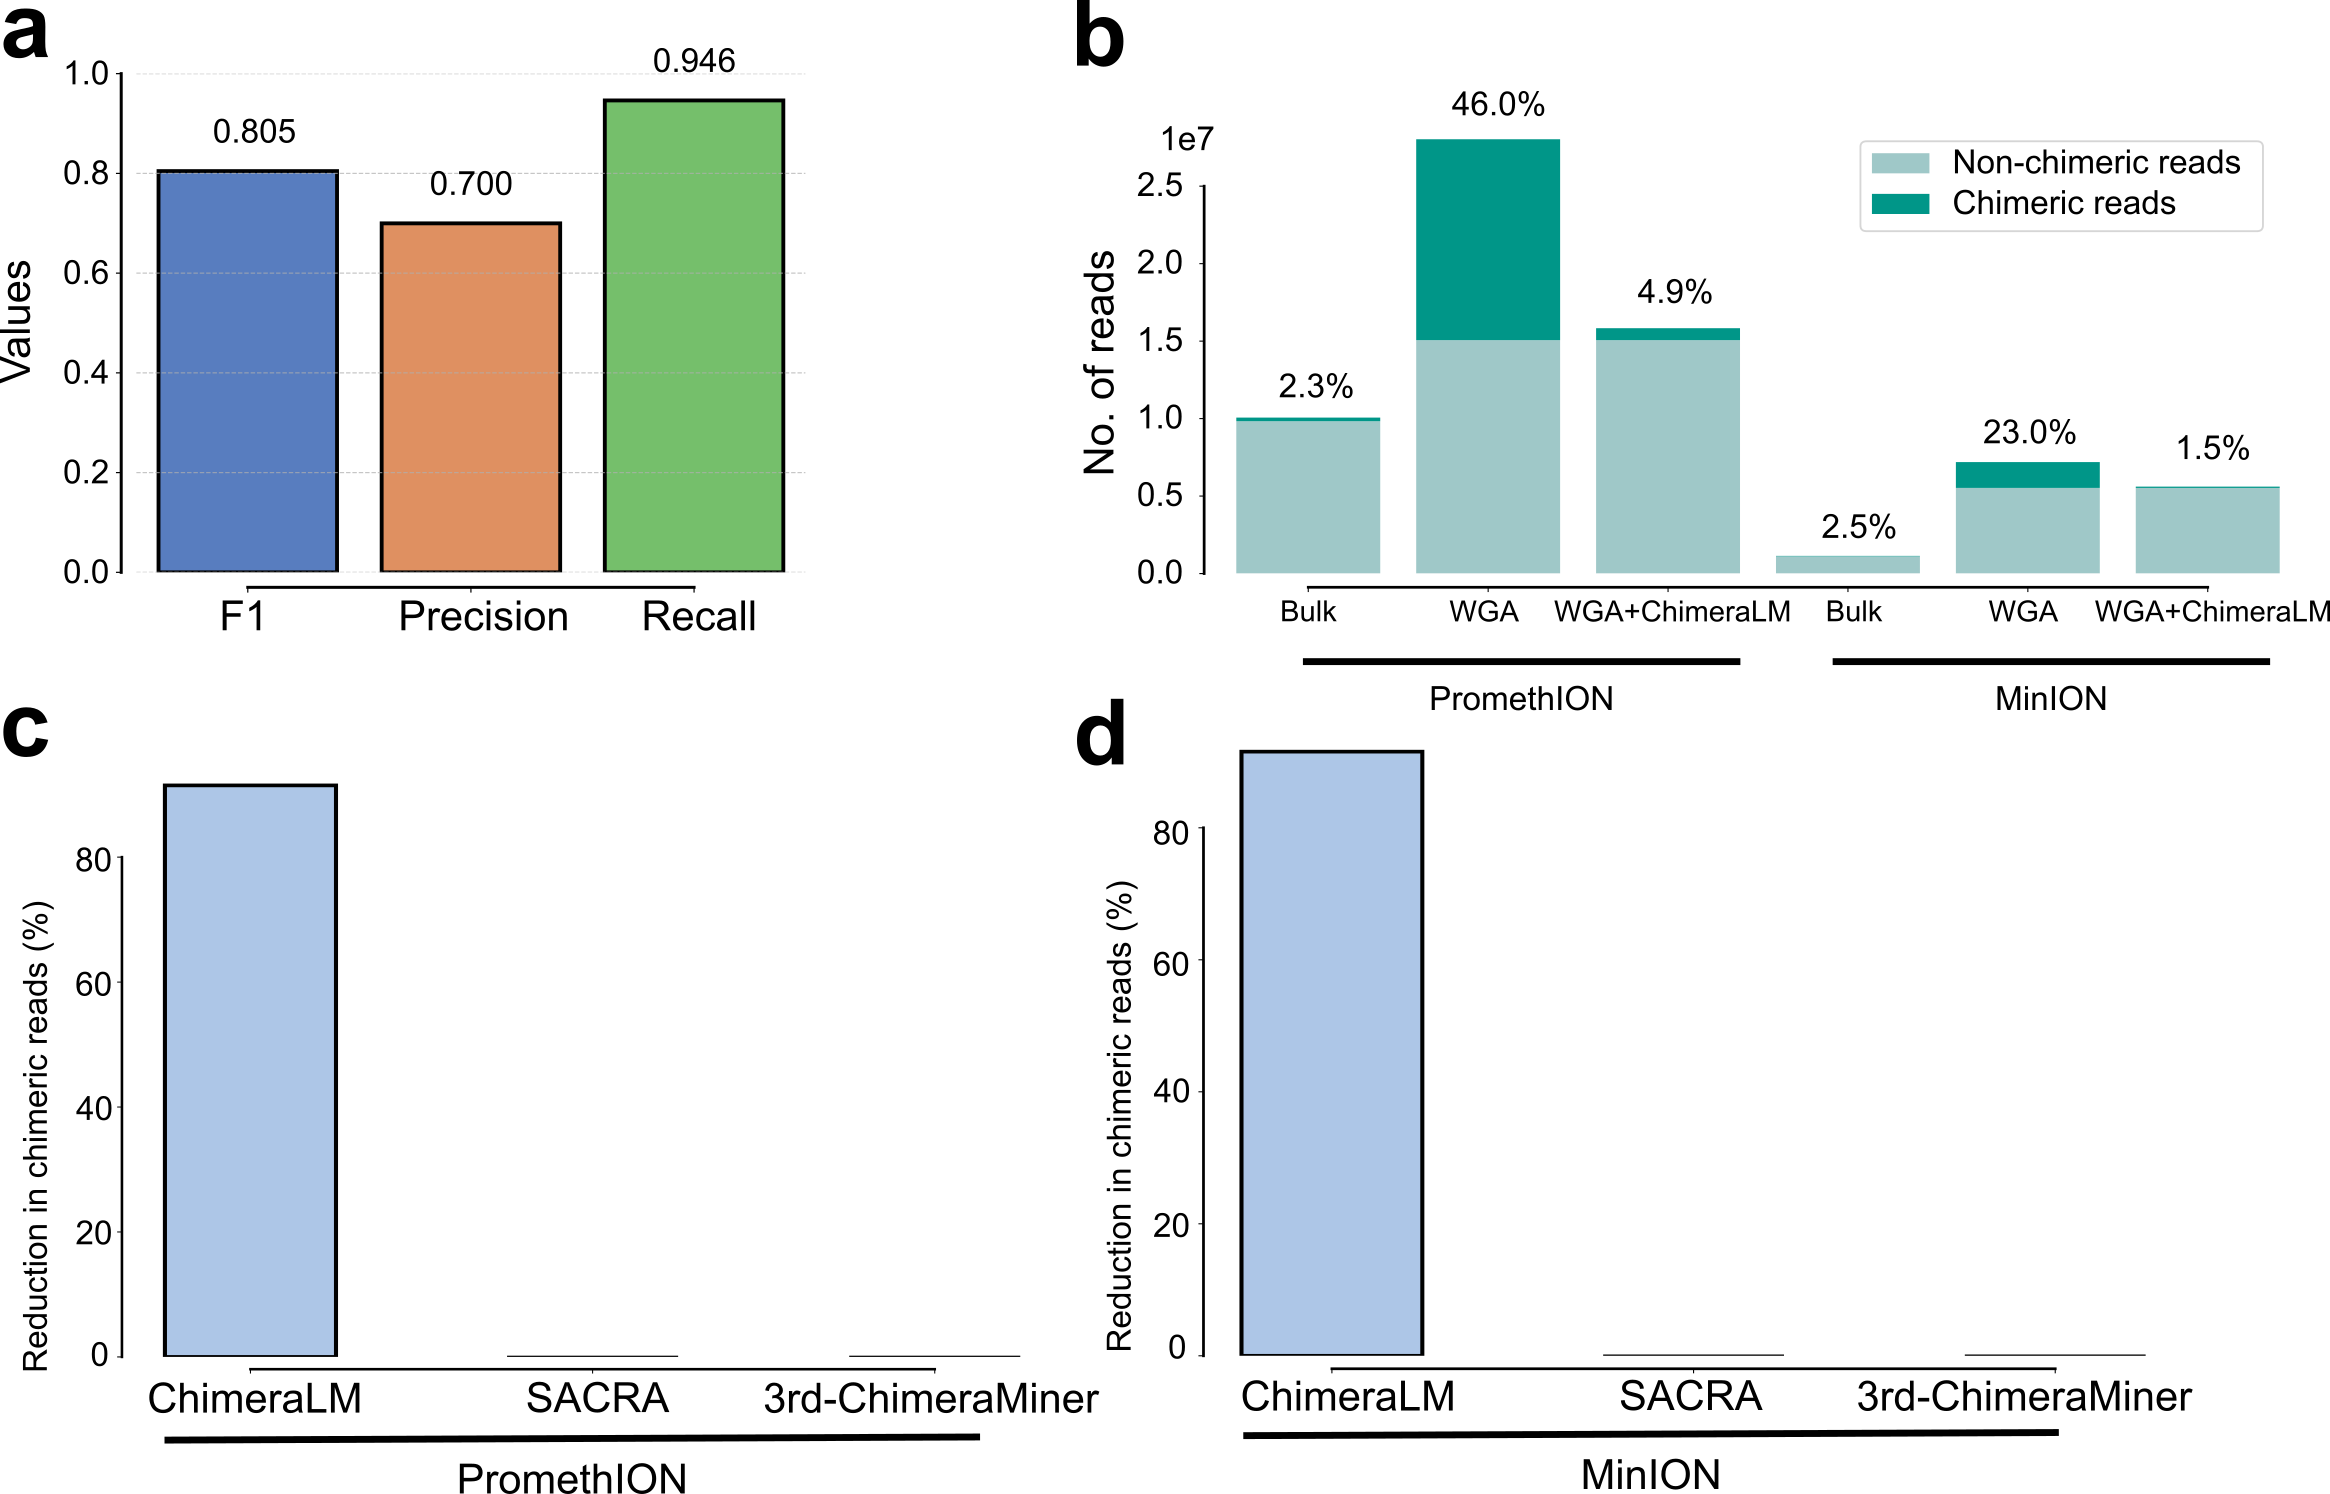
\includegraphics[width=0.95\textwidth]{final_figures/figure2}
	\end{center}
	\caption{{\bf ChimeraLM performance evaluation and benchmarking against existing methods.}
		(a) ChimeraLM performance metrics on test dataset. Bar chart showing F1 score (0.805), precision (0.700), and recall (0.946) achieved by ChimeraLM on held-out test data for binary classification of biological versus chimeric artifacts.
		(b) Chimeric read reduction across sequencing platforms. Stacked bar charts comparing chimeric read proportions (dark teal) versus non-chimeric reads (light teal) across bulk sequencing, \gls{wga}, and ChimeraLM-processed samples for PC3 cell line data. Left panel shows PromethION P2 platform data with chimeric rates of 2.3\% (bulk), 46.0\% (\gls{wga}), and 4.9\% (ChimeraLM). Right panel shows MinION Mk1c platform data with chimeric rates of 2.5\% (bulk), 23.0\% (\gls{wga}), and 1.5\% (ChimeraLM).
		(c) Benchmarking on P2 platform data. Bar chart showing percentage reduction in chimeric reads achieved by ChimeraLM ($\sim$92\%) compared to existing computational methods SACRA and 3rd-ChimeraMiner (both 0\% reduction).
		(d) Benchmarking on Mk1c platform data. Bar chart showing percentage reduction in chimeric reads achieved by ChimeraLM ($\sim$91\%) compared to SACRA and 3rd-ChimeraMiner (both 0\% reduction).}\label{fig:figure2}
\end{figure}

\subsection*{ChimeraLM achieves high performance in chimeric artifact detection}

We evaluated ChimeraLM's performance on held-out test data to assess its ability to accurately classify biological and chimeric reads (Fig.~\ref{fig:figure2}a).
ChimeraLM demonstrated robust performance across key classification metrics, achieving an F1 score of 0.805, which balances precision and recall for the binary classification task.
The model exhibited high recall of 0.946, indicating that it successfully identified 94.6\% of true chimeric artifacts in the test dataset, minimizing the risk of retaining false-positive structural variants in downstream analyses.
The precision of 0.700 demonstrates that 70.0\% of reads classified as chimeric were indeed artifacts, representing a trade-off that prioritizes comprehensive artifact removal while maintaining reasonable specificity.

\subsection*{ChimeraLM reduces chimeric artifact burden across sequencing platforms}

To evaluate ChimeraLM's practical impact, we applied the trained model to PC3 cell line data generated on two Nanopore long-read sequencing platforms: PromethION P2 and MinION Mk1c (Fig.~\ref{fig:figure2}b).
The analysis revealed substantial differences in chimeric read proportions between bulk sequencing, \gls{wga} samples, and ChimeraLM-processed data.

For P2 platform data, bulk sequencing exhibited a low baseline chimeric rate of 2.3\% among 10,065,403 total reads, consistent with the expected minimal artifact rate in non-amplified samples.
In contrast, \gls{wga} amplification dramatically increased the chimeric burden to 46.0\% of reads in a dataset containing 28,027,667 total sequences.
ChimeraLM processing effectively reduced this chimeric proportion to 4.9\% while retaining 15,833,834 high-quality biological reads, representing a $\sim$10-fold reduction in artifact contamination compared to unprocessed \gls{wga} data.

Similar results were observed for Mk1c platform data, where bulk sequencing contained 2.5\% chimeric reads among 1,140,363 total sequences.
\gls{wga} amplification increased chimeric contamination to 23.0\% of 7,193,945 total reads.
ChimeraLM processing reduced the chimeric fraction to 1.5\% while preserving 5,610,252 biological reads, achieving nearly complete artifact removal that approached the quality of bulk sequencing data.

These results demonstrate ChimeraLM's effectiveness across different Nanopore sequencing platforms and highlight the substantial chimeric artifact burden introduced by \gls{wga}, which varies between platforms but is consistently and dramatically reduced by ChimeraLM processing.

\subsection*{ChimeraLM outperforms existing chimera artifact detection tools}

We benchmarked ChimeraLM against established computational methods for chimeric sequence detection, including SACRA~\cite{kiguchi2021long} and 3rd-ChimeraMiner~\cite{lu2023exploration}, using both P2 and Mk1c datasets (Fig.~\ref{fig:figure2}c,d).
ChimeraLM achieved superior performance compared to existing approaches across both sequencing platforms.

For P2 data, ChimeraLM reduced chimeric read contamination by $\sim$92\%, demonstrating substantial improvement in data quality (Fig.~\ref{fig:figure2}c).
In contrast, both SACRA and 3rd-ChimeraMiner failed to achieve meaningful chimeric read reduction, showing 0\% improvement over unprocessed \gls{wga} data.
This stark difference highlights the limitations of existing rule-based and alignment-based approaches for detecting complex chimeric artifacts in long-read sequencing data.

Similar performance advantages were observed for Mk1c data, where ChimeraLM again achieved $\sim$91\% reduction in chimeric reads while SACRA and 3rd-ChimeraMiner provided no detectable improvement (Fig.~\ref{fig:figure2}d).
These results demonstrate that ChimeraLM's deep learning approach captures complex sequence patterns that are not effectively identified by traditional computational methods.

The consistent superior performance across different sequencing platforms establishes ChimeraLM as a significant advance over existing tools, providing researchers with a reliable method for improving single-cell genomic data quality regardless of the specific long-read sequencing technology employed.

\begin{figure}[!ht]
	\begin{center}
		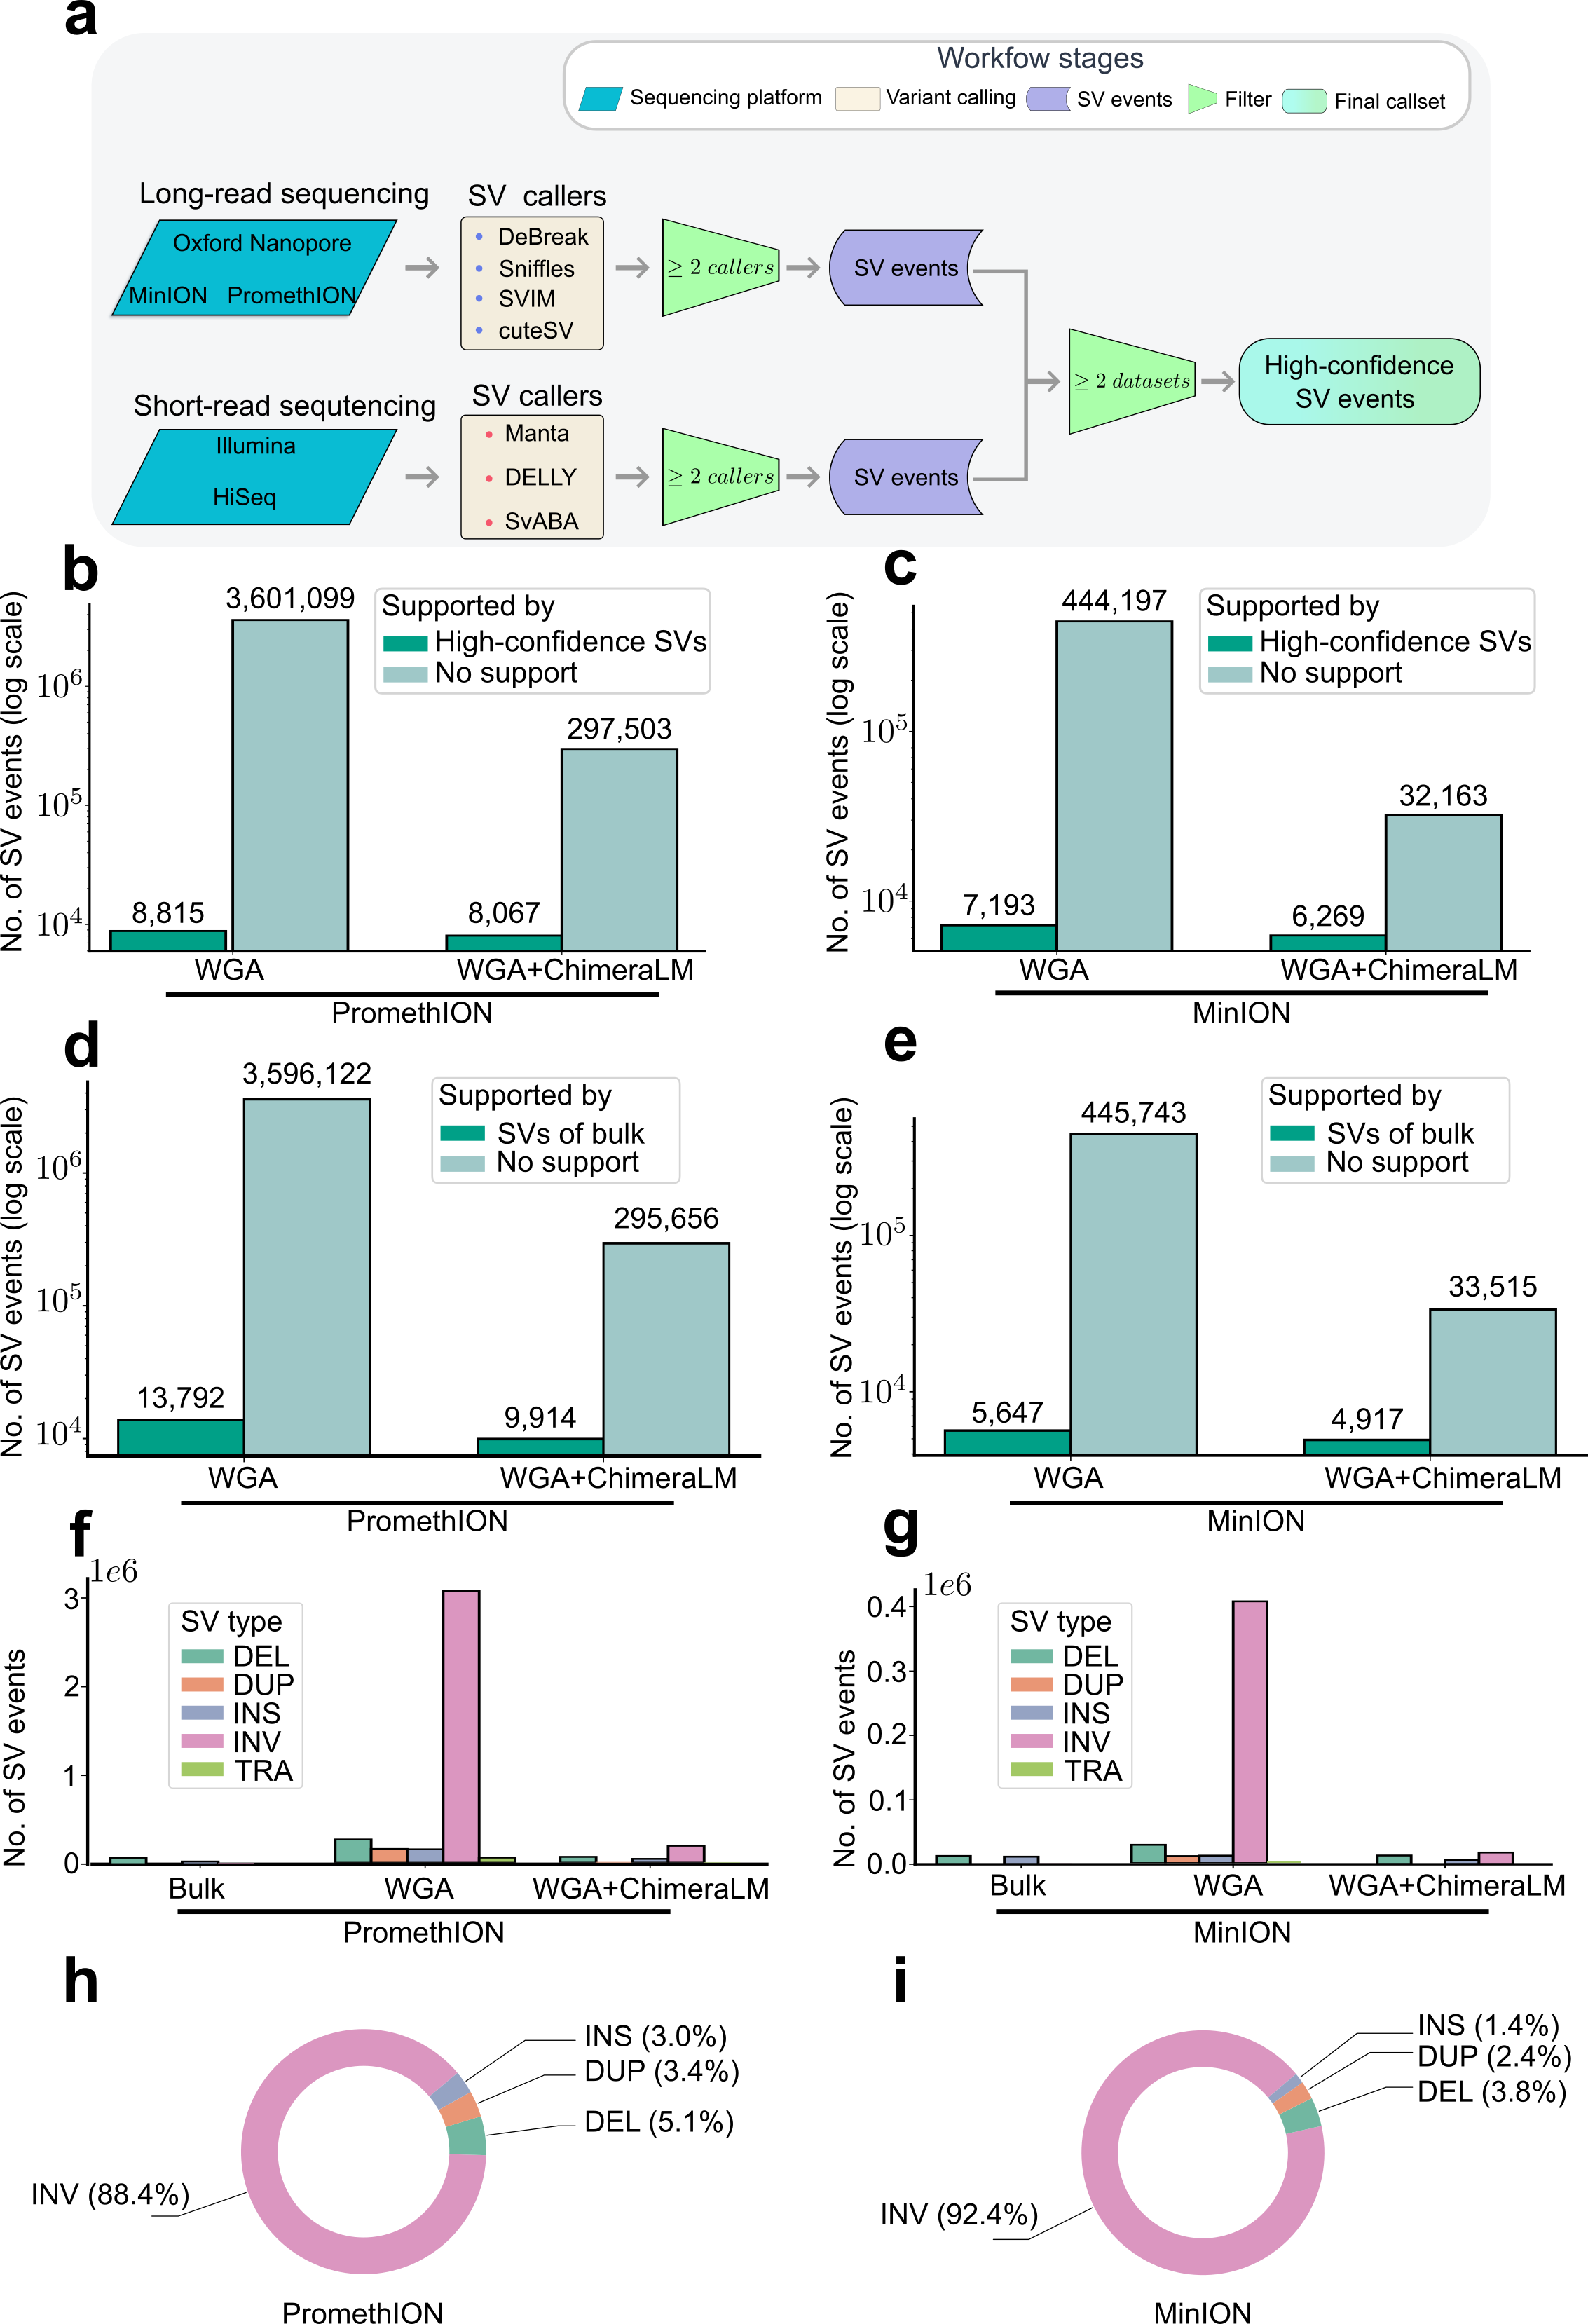
\includegraphics[width=0.95\textwidth]{final_figures/figure3}
	\end{center}
	\caption{{\bf \gls{sv} detection accuracy and type distribution analysis.}
		(a) Workflow for constructing gold standard \gls{sv} dataset from bulk sequencing data. Long-read sequencing (Oxford Nanopore Mk1c and P2) and short-read sequencing (Illumina HiSeq) platforms are used with multiple \gls{sv} callers. \gls{sv} events detected by $\geq$2 callers per platform are filtered, and events supported by $\geq$2 datasets (both long-read and short-read) are retained as high-confidence \gls{sv} events for gold standard.
		(b,c) \gls{sv} validation using bulk sequencing gold standard. Stacked bar charts showing total \gls{sv} calls (log scale) classified as supported (dark teal) or unsupported (light teal) events when compared against gold standard. Panel (b) shows PromethION P2 results comparing \gls{wga} vs ChimeraLM-filtered data; panel (c) shows MinION Mk1c results. Numbers above bars indicate absolute counts of supported/unsupported events.
		(d,e) \gls{sv} type distributions across sample processing methods. Bar charts displaying the number of detected structural variants by type: \gls{del} (green), \gls{dup} (orange), \gls{ins} (blue), \gls{inv} (pink), and \gls{tra} (light green). Panel (d) shows P2 platform data; panel (e) shows Mk1c platform data. Data compared across bulk sequencing, ChimeraLM-filtered, and unfiltered \gls{wga} samples.
		(f,g) Composition of chimeric artifact-supported \gls{sv}. Pie charts showing the proportion of different \gls{sv} types among events supported specifically by reads classified as chimeric artifacts by ChimeraLM in unfiltered \gls{wga} data. Panel (f) shows P2 data; panel (g) shows Mk1c data. Percentages indicate relative frequency of each \gls{sv} class within the chimeric artifact-supported subset.}\label{fig:figure3}
\end{figure}

\subsection*{ChimeraLM improves structural variant calling accuracy by reducing false positives}

To evaluate ChimeraLM's impact on downstream structural variant analysis, we constructed a gold-standard \gls{sv} dataset using bulk sequencing data (Fig.~\ref{fig:figure3}a) and assessed \gls{sv} detection performance on both P2 and Mk1c platforms with and without ChimeraLM filtering (Fig.~\ref{fig:figure3}b,c).
The gold standard was constructed by integrating long-read (Nanopore P2 and Mk1c) and short-read (Illumina HiSeq) sequencing platforms with multiple \gls{sv} callers, retaining only high-confidence events supported by $\geq$2 callers per platform and $\geq$2 datasets (Fig.~\ref{fig:figure3}a).
This analysis directly measures ChimeraLM's ability to improve the biological relevance of \gls{sv} calls by comparing detected events against high-confidence reference data.

For P2 platform data, unprocessed \gls{wga} samples yielded 3,609,914 total structural variant calls, of which only 8,815 (0.24\%) were supported by the gold standard (Fig.~\ref{fig:figure3}b).
The remaining 3,601,099 calls represented unsupported events likely arising from chimeric artifacts and other amplification biases.
ChimeraLM processing dramatically improved this ratio, reducing total \gls{sv} calls to 305,570 while maintaining 8,067 supported events (2.64\% of total calls).
This represents a $\sim$12-fold increase in validation rate while preserving 91.5\% of true positive events, compared with \gls{wga} data.

Similar improvements were observed for Mk1c data, where raw \gls{wga} processing identified 451,390 total \gls{sv} with 7,193 supported events (1.59\%) (Fig.~\ref{fig:figure3}c).
ChimeraLM filtering reduced the total to 38,432 calls while retaining 6,269 supported events, achieving a 16.3\% validation rate ($\sim$10-fold increase) and preserving 87.2\% of true positive \gls{sv} compared with \gls{wga} data.
The consistent performance across platforms demonstrates ChimeraLM's robust ability to eliminate false-positive \gls{sv} while maintaining detection sensitivity for genuine genomic alterations.

\subsection*{ChimeraLM normalizes structural variant type distributions toward bulk sequencing profiles}

We analyzed the distribution of \gls{sv} types to assess whether ChimeraLM processing restores \gls{sv} profiles characteristic of high-quality bulk sequencing data (Fig.~\ref{fig:figure3}d,e).
This analysis tests the hypothesis that \gls{wga} introduces systematic biases in the apparent frequency of different \gls{sv} classes, which should be corrected by effective chimeric artifact removal.

In both P2 and Mk1c datasets, bulk sequencing exhibited balanced distributions across \gls{del}, \gls{dup}, \gls{ins}, \gls{inv}, and \gls{tra} events, with relatively modest numbers reflecting the stringent quality filtering applied to establish the gold standard (Fig.~\ref{fig:figure3}d,e).
Unprocessed \gls{wga} data showed dramatically skewed distributions dominated by spurious \gls{inv} events, consistent with literature reports that \gls{inv} are frequently artificial in amplified samples due to template switching during \gls{wga}~\cite{lu2023exploration, lu2023chimera}.

ChimeraLM processing substantially normalized these distributions, reducing the overwhelming preponderance of false-positive \gls{inv} while maintaining more balanced representation of other \gls{sv} types.
The filtered data profiles more closely resembled bulk sequencing distributions, indicating that ChimeraLM successfully identifies and removes the systematic biases introduced by \gls{wga} without eliminating legitimate \gls{sv} of other classes.

\subsection*{Characterization of chimeric artifact-supported false-positive structural variants}

To understand the specific types of false-positive \gls{sv} that would be retained without ChimeraLM filtering, we analyzed the \gls{sv} events in unfiltered \gls{wga} data that were specifically supported by reads classified as chimeric artifacts by ChimeraLM (Fig.~\ref{fig:figure3}f,g).
This analysis profiles the "false-positive landscape" that researchers would encounter without effective chimeric artifact removal.

For P2 data, chimeric artifact-supported \gls{sv} were overwhelmingly dominated by \gls{inv} (88.4\% of events), with smaller contributions from \gls{del} (5.1\%), \gls{dup} (3.4\%), and \gls{ins} (3.0\%) (Fig.~\ref{fig:figure3}f).
This extreme bias toward inversions confirms that template switching during \gls{wga} predominantly manifests as apparent \gls{inv} events in downstream \gls{sv} calling pipelines.

Mk1c data showed a similar but even more pronounced pattern, with \gls{inv} comprising 92.4\% of chimeric artifact-supported events, followed by \gls{del} (3.8\%), \gls{dup} (2.4\%), and \gls{ins} (1.4\%) (Fig.~\ref{fig:figure3}g).
The consistency of this pattern across platforms indicates that inversion artifacts represent the primary mode of false-positive \gls{sv} generation in \gls{wga} workflows.

These results demonstrate that without ChimeraLM, genomic studies would be severely compromised by false-positive \gls{inv} calls, potentially leading to misinterpretation of chromosomal instability, copy number profiles, and other key genomic features.
ChimeraLM's ability to identify and remove these specific artifacts represents a critical advancement for accurate \gls{sv} analysis.

\subsection*{ChimeraLM predictions correlate with chimeric alignment complexity}

To validate ChimeraLM's classification accuracy, we analyzed the distribution of chimeric alignments per chimeric read, comparing how ChimeraLM classified these known chimeric sequences as biological versus artificial (Extended Data Fig.~\ref{fig:sf2}a,b).
This provides independent validation by examining whether ChimeraLM correctly identifies the most structurally complex chimeric artifacts.

Among chimeric reads, those classified as "artificial" by ChimeraLM predominantly exhibited 2 chimeric alignments per read ($\sim$1.0 $\times$ 10$^7$ and $\sim$1.4 $\times$ 10$^6$ reads in P2 and Mk1c data, respectively), representing simple two-part chimeric structures.
Smaller fractions showed 3+ alignments ($\sim$2.1 $\times$ 10$^6$ and $\sim$0.2 $\times$ 10$^6$ reads in P2 and Mk1c data, respectively), indicating more complex multi-fragment chimeras from sequential template switching events.

Importantly, chimeric reads classified as "biological" by ChimeraLM showed minimal representation across all alignment complexity categories, suggesting these may represent genuine structural variants or less disruptive chimeric events that preserve biological relevance.

This pattern demonstrates that ChimeraLM successfully prioritizes the most structurally complex and potentially problematic chimeric artifacts for removal, while preserving chimeric reads that may still retain biological information.
The consistency across both datasets validates ChimeraLM's ability to distinguish between different classes of chimeric complexity.

\begin{figure}[!ht]
	\begin{center}
		\includegraphics[width=\textwidth]{final_figures/figure4}
	\end{center}
	\caption{{\bf Attention-based interpretability reveals ChimeraLM's capacity to focus on chimeric junction regions.}
		(a) Attention weight profile across a representative chimeric read. Upper panel shows attention weights per sequence position (blue line) with overall mean attention (dashed line). Red vertical line indicates the chimeric junction position in the read, with pink shading marking the junction window ($\pm$50 bp). Purple arrow indicates the corresponding \gls{sv} breakpoint position in the reference genome. Lower panel illustrates read alignment: the read (top bar) shows reverse-complemented sequence (red with leftward arrows) transitioning to forward sequence (green with rightward arrows) at the junction. Reference genome (bottom bar) shows continuous forward orientation, with gray regions indicating alignment relationships.
		(b) Quantitative comparison of attention weights between junction window and background regions. Box plots show significantly elevated attention weights in the junction window (median $\sim$0.0008) compared to background regions (median $\sim$0.0003), with statistical significance indicated (***, $p < 0.001$, Wilcoxon rank-sum test).
		(c) Proposed mechanism of chimera formation during \gls{wga}. Step 1: Original DNA fragments from distant genomic loci (Fragment A and Fragment B) exist in forward orientation. Step 2: During \gls{wga}, Fragment A undergoes random reverse-complementation while Fragment B maintains forward orientation. Step 3: Template switching causes artificial joining of the two fragments, creating a chimeric artifact with discordant orientation patterns.}\label{fig:figure4}
\end{figure}

\subsection*{ChimeraLM demonstrates capacity to learn biologically relevant sequence features}

To investigate whether ChimeraLM can capture biologically meaningful features for chimeric artifact detection, we examined the attention weight distributions from the model's pooling mechanism.
Attention weights indicate which sequence regions contribute most strongly to individual classification decisions, providing potential insight into learned patterns.

We present representative examples where ChimeraLM's attention mechanism shows focused activity at chimeric junction sites (Fig.~\ref{fig:figure4} and Extended Data Fig.~\ref{fig:sf3}).
In these chimeric reads, the attention profiles exhibited predominantly low baseline weights with pronounced peaks coinciding with chimeric junctions where reads transition between reverse-complemented and forward-oriented sequences.
These junctions represent artificial joining points where DNA fragments from different genomic loci were ligated during \gls{wga}.

The alignment pattern illustrates the structural signature present in these examples (Fig.~\ref{fig:figure4}a).
In the first example, the read portion aligns in reverse orientation (red), while the downstream portion aligns in forward orientation to a distant genomic location (green).
This discordant orientation pattern represents a characteristic feature of \gls{wga}-induced chimeric artifacts.

For these specific examples, quantitative analysis showed that attention weights within 100 bp windows ($\pm$50 bp) centered on chimeric junctions exhibited significantly higher values compared to background regions (Fig.~\ref{fig:figure4}b).
The median attention weight in the junction window was approximately 2.7-fold higher than background (window median: 0.0008; background median: 0.0003; $p < 0.001$, Wilcoxon rank-sum test).

These examples align with the proposed mechanism of chimera formation during \gls{wga} (Fig.~\ref{fig:figure4}c).
Original DNA fragments from distant genomic loci undergo random orientation changes during amplification.
Template switching events cause these independently oriented fragments to be artificially joined, creating chimeric constructs with orientation discontinuities at junction sites.

These case studies demonstrate that ChimeraLM has the capacity to learn biologically interpretable features related to chimeric junction sites, though the prevalence and consistency of this attention pattern across the full dataset remains to be systematically characterized.
The observation that the model can focus on mechanistically relevant sequence features in at least some cases provides evidence that ChimeraLM's learned representations may incorporate structural signatures of \gls{wga} artifacts rather than relying solely on other sequence characteristics.

\section*{Discussion}
ChimeraLM addresses a fundamental bottleneck that has limited the widespread adoption and reliability of single-cell genomic approaches.
While \gls{wga} has enabled genomic analysis of individual cells, the systematic introduction of chimeric artifacts has remained an unsolved challenge that compromises downstream interpretations and limits biological insights.

Traditional approaches to managing \gls{wga} artifacts have focused on post-hoc filtering of \gls{sv} calls or coverage-based correction methods~\cite{kiguchi2021long, lu2023exploration}.
ChimeraLM represents a paradigm shift toward proactive identification of problematic sequences before they impact downstream analyses.
This upstream intervention strategy addresses the root cause of analytical errors rather than attempting to correct their consequences after variant calling.

The success of this approach demonstrates the power of modern genomic language models to capture complex sequence patterns that are not readily apparent through traditional bioinformatics methods.
Unlike rule-based approaches that rely on predefined criteria, ChimeraLM learns directly from data, enabling discovery of subtle features that distinguish authentic biological sequences from amplification artifacts~\cite{lu2023exploration, agyabeng2025evaluating, nguyen2023hyenadna}.
This data-driven approach is particularly valuable for complex genomic phenomena where explicit rules may be insufficient or unknown.

The demonstrated effectiveness of ChimeraLM has broader implications for single-cell genomics methodology.
The ability to substantially improve data quality through computational approaches reduces the experimental burden of optimizing amplification protocols and may enable researchers to focus on biological questions rather than technical optimization.
This could accelerate adoption of single-cell genomic approaches in laboratories with limited specialized expertise in amplification chemistry.

Furthermore, improved reliability of \gls{sv} detection opens new avenues for applications that have been previously constrained by high false-positive rates.
Studies of chromosomal instability, copy number evolution, and \gls{sv} burden in individual cells become more feasible when researchers can have confidence in the authenticity of detected events.

ChimeraLM's success exemplifies the transformative potential of language model approaches in genomics.
The recent emergence of foundation models for biological sequences has demonstrated remarkable capabilities across diverse tasks, but most applications have focused on prediction of molecular phenotypes or functional annotations.
ChimeraLM represents one of the first applications of \gls{glm} to quality control and data preprocessing, suggesting that these approaches may have broader utility for improving experimental data quality than previously recognized.

The architectural innovations incorporated in ChimeraLM, particularly the use of Hyena operators for efficient long-range modeling, may have applications beyond chimeric detection~\cite{Poli2023HyenaHT, nguyen2023hyenadna}.
Similar approaches could potentially address other quality control challenges in genomics, such as contamination detection, adapter artifact identification, or systematic error correction in diverse sequencing technologies.

While ChimeraLM represents a significant advance, several limitations merit consideration.
The requirement for paired bulk sequencing data for training constrains the initial application scope, though this limitation may be addressable through transfer learning approaches as the method matures.
The current focus on Nanopore platforms, while representing the most common long-read technology for single-cell applications, leaves questions about broader platform compatibility.

More fundamentally, the binary classification approach assumes a clear distinction between biological and artificial sequences.
In reality, some chimeric events may represent genuine biological phenomena, such as chromothripsis or complex structural rearrangements.
Future developments may need to incorporate more nuanced classification schemes that can distinguish between different types of chimeric events based on their likely biological relevance.

The success of ChimeraLM suggests several promising directions for future development.
Integration with real-time sequencing platforms could enable immediate quality assessment and adaptive sampling strategies.
Extension to other single-cell genomic applications, such as chromatin accessibility or methylation analysis, could address analogous quality control challenges in emerging single-cell methods.

The interpretability features of modern language models could be leveraged to provide insights into the sequence features that distinguish chimeric artifacts, potentially informing development of improved amplification protocols.
This feedback loop between computational analysis and experimental optimization could drive continuous improvement in single-cell genomic methods.

ChimeraLM demonstrates that sophisticated computational approaches can effectively address fundamental technical challenges that have limited single-cell genomics.
By providing a robust solution to chimeric artifact detection, this work removes a significant barrier to reliable single-cell genomic analysis and opens new possibilities for biological discovery and clinical application.
As single-cell approaches become increasingly central to modern biology and medicine, computational tools like ChimeraLM will be essential for realizing their full potential.

\section*{Methods}\label{sec:methods}

\subsection*{MDA sequencing}

\subsection*{Sequencing and data processing}

\paragraph{Sequencing platforms}
Long-read sequencing was performed using Oxford Nanopore Technologies platforms, including PromethION P2 and MinION Mk1c devices.
Both \gls{wga}-amplified and bulk (non-amplified) DNA samples from PC3 cell line were sequenced to generate paired datasets for training and evaluation.
Sequencing libraries were prepared following manufacturer's protocols for genomic DNA sequencing.

\paragraph{Read alignment and processing}
Raw sequencing reads were basecalled and quality-filtered using standard Nanopore basecalling pipelines.
Reads were aligned to the human reference genome (GRCh38/hg38) using minimap2~\cite{li2018minimap2} with parameters optimized for long-read genomic alignment (-ax map-ont).
Alignment files were processed using SAMtools~\cite{danecek2021twelve} for sorting, indexing, and quality filtering.

\paragraph{Chimeric read identification}
Chimeric reads were identified based on the presence of supplementary alignments in BAM files using the SA (Supplementary Alignment) tag.
The SA tag indicates that a read has additional alignments beyond the primary alignment, which is characteristic of chimeric sequences that map to multiple distant genomic locations.
Reads containing the SA tag were classified as chimeric reads, while reads without the SA tag (single continuous alignments) were classified as non-chimeric.
This approach leverages the standard BAM format specification to reliably identify reads with complex alignment patterns.

\subsection*{Training data construction}

\paragraph{Paired sequencing dataset generation}
Training data for ChimeraLM was constructed using a novel comparative approach that leverages paired \gls{wga} and bulk sequencing datasets from identical biological samples (PC3 cell line).
This methodology exploits the fundamental difference between amplified and non-amplified samples to establish reliable ground truth labels for supervised learning.
Bulk sequencing data serves as a reference standard containing only genuine biological sequences, while \gls{wga} data contains both authentic genomic content and amplification-induced chimeric artifacts.
Sample preparation involved processing PC3 cell line to generate matched \gls{wga} and bulk sequencing datasets.

\paragraph{Ground truth labeling methodology}
The core innovation of our training data construction lies in the comparative labeling strategy that automatically generates binary classification labels.
Each chimeric read from the \gls{wga} dataset was systematically compared against the corresponding bulk sequencing data through sequence alignment analysis to determine its biological authenticity.

Chimeric reads from \gls{wga} data were compared against the bulk sequencing dataset to identify chimera present in both datasets.
\gls{wga} reads that successfully aligned to bulk sequences were classified as biological, indicating they represent authentic genomic content preserved through the amplification process.
Conversely, \gls{wga} reads that failed to align to any chimeric sequences in the bulk dataset were labeled as artificial chimeric artifacts, representing spurious sequences generated during the amplification process.
The comparison-based classification approach ensures that training labels reflect objective evidence of sequence authenticity.
This methodology captures the full spectrum of naturally occurring chimeric artifacts while providing reliable positive examples of biological sequences that successfully traverse the amplification process.

\paragraph{Dataset partitioning and stratification}
The complete labeled dataset was partitioned into training, validation, and test sets using stratified sampling to maintain balanced representation of biological and artificial sequences across all data splits.
The training set comprised 70\% of the total data and was used for model parameter optimization during supervised learning.
The validation set contained 20\% of the data and served for hyperparameter tuning, model selection, and monitoring training progress.
The remaining 10\% was reserved as a held-out test set for final performance evaluation and remained completely isolated from the training process.

Stratification ensured that each data partition maintained similar proportions of biological and artificial sequences, preventing training bias that could arise from imbalanced class distributions. Random sampling within strata was employed to minimize systematic biases while maintaining statistical representativeness of the overall dataset characteristics.

\subsection*{Model architecture}

ChimeraLM uses a pre-trained HyenaDNA which provides robust genomic sequence representations learned from large-scale genomic data.
The backbone model handles DNA sequence tokenization using single base pair resolution, converting nucleotide sequences into token representations.

Input sequences are processed through the Hyena operators.
The backbone generates contextualized hidden representations for each position in the input sequence, capturing both local sequence motifs and long-range dependencies essential for distinguishing biological sequences from chimeric artifacts.

ChimeraLM employs a binary sequence classifier designed specifically for genomic sequence classification tasks.
The classification head processes the hidden states through a multi-stage architecture optimized for variable-length sequence classification.
The classifier implements attention-based pooling to aggregate variable-length sequence representations into fixed-size feature vectors.
$$
	\textrm{attention\_weights} = \textrm{softmax}(\textrm{Linear}(\textrm{GELU}(\textrm{Linear}(\textrm{hidden\_states}))))
$$
The attention pooling mechanism computes position-wise attention weights through a two-layer neural network where the first linear layer projects from the hidden dimension to 256 dimensions, followed by \gls{gelu} activation and a second linear layer projecting to a single attention score per position.
The attention weights are normalized using \emph{softmax} and applied to compute the weighted sum of hidden states across sequence positions.
When attention masks are provided for variable-length sequences, the attention weights are masked to exclude padding tokens and renormalized to ensure proper probability distribution over valid sequence positions.
This approach accommodates the natural variability in sequencing read lengths without introducing computational inefficiency or artificial sequence information.

The pooled sequence representation is processed through a \gls{mlp} with residual connections.
The \gls{mlp} uses two hidden layers, each consisting of linear transformation to 512 hidden dimensions, \gls{gelu} activation function, and dropout regularization with rate 0.1.
This residual design enables stable gradient flow during training and improved representation learning for complex genomic patterns.

The final classification layer maps the processed features to binary classification logits using a linear transformation with output dimension 2.
The model outputs two logits corresponding to biological and artificial classes rather than a single probability, enabling the use of cross-entropy loss during training.
Classification predictions are made by selecting the class with the highest logit value.

\subsection*{Model training and optimization}

\paragraph{Training data preparation}
ChimeraLM was trained using the paired \gls{wga} and bulk sequencing dataset constructed from PromethION P2 platform data.
The tokenizer was initialized from the pre-trained HyenaDNA model to maintain consistency with the backbone architecture and preserve the benefits of pre-training on large-scale genomic data.
This approach ensures that input sequences are processed using the same tokenization scheme employed during the backbone model\textquotesingle{s} original training, enabling effective transfer learning for the chimeric detection task.

\paragraph{Model training framework and optimization}
Model training was implemented within PyTorch~\cite{paszke2019pytorch} and PyTorch Lightning framework~\cite{Falcon_PyTorch_Lightning_2019}, providing a standardized interface for supervised classification tasks with automatic handling of training loops, validation procedures, and model checkpointing.
The training process employed mixed-precision computation using bf16-mixed precision to accelerate training while maintaining numerical stability for gradient computation.

The optimization procedure utilized the AdamW optimizer~\cite{adamw}, an extension of the Adam optimizer~\cite{kingma2014adam} that incorporates decoupled weight decay regularization.
The optimizer was configured with a learning rate of $1\times10^-4$ and weight decay coefficient of 0.01.
The AdamW optimizer updates model parameters $\theta$ according to the following formulation:
$$
	\theta_{t+1} = \theta_t - \alpha \left( \frac{\hat{m}_t}{\sqrt{\hat{v}_t} + \epsilon} + \lambda \theta_t \right)
$$
where $\alpha$ represents the learning rate, $\hat{m}_t$ and $\hat{v}_t$ are bias-corrected first and second moment estimates, $\epsilon$ is a small constant for numerical stability, and $\lambda$ denotes the weight decay coefficient.
The decoupled weight decay term $\lambda \theta_t$ provides regularization that is independent of the gradient-based updates.

Early stopping was implemented with a patience of 10 epochs to prevent over-fitting and automatically terminate training when validation performance ceased to improve.
This approach ensures optimal model generalization by identifying the point of best validation performance rather than training to completion.
The training process used a fixed random seed of 12345 to ensure reproducibility across multiple training runs and facilitate comparison of different model configurations.

\paragraph{Loss function and objective formulation}
The training objective employed cross-entropy loss for the binary classification task, providing probabilistically grounded optimization that encourages the model to produce well-calibrated probability estimates.
For a training example with true class label $y \in \{0,1\}$ and model output logits $z = [z_0, z_1]$, the cross-entropy loss is computed as:
$$
	\mathcal{L} = -\log(\textrm{softmax}(z_y)) = -\log\left(\frac{\exp(z_y)}{\exp(z_0) + \exp(z_1)}\right)
$$
where the softmax function converts logits to normalized probability distributions over the two classes (biological and artificial).
The cross-entropy formulation provides strong gradients for misclassified examples while allowing confident predictions to contribute minimal loss, enabling efficient learning of the decision boundary between biological sequences and chimeric artifacts.

\paragraph{Data loading and computational configuration}
Training employed a batch size of 48 sequences per batch, balancing computational efficiency with memory constraints and gradient stability.
Data loading was optimized using 30 parallel workers to minimize I/O bottlenecks and ensure continuous data supply to the \gls{gpu} during training.

The training infrastructure utilized \gls{gpu} acceleration (two A100 \glspl{gpu}) to enable efficient processing of the large-scale genomic sequence datasets.
Mixed-precision training with brain floating-point 16-bit (bf16) format was employed to reduce memory requirements and accelerate computation while maintaining numerical precision sufficient for stable gradient computation and model convergence.

\paragraph{Model validation and evaluation}
Model performance was continuously monitored throughout training using the validation dataset.
The model evaluation metrics included accuracy, precision, recall and the F1 score, calculated using the following equations:
\begin{align*}
	\textrm{Precision} & = \frac{\textrm{TP}}{\textrm{TP}+\textrm{FP}}                                                     \\
	\textrm{Recall}    & = \frac{\textrm{TP}}{\textrm{TP}+\textrm{FN}}                                                     \\
	\textrm{F1}        & = 2 \times \frac{\textrm{Precision} \times \textrm{Recall}}{\textrm{Precision} + \textrm{Recall}} \\
	\textrm{Accuracy}  & = \frac{\textrm{TP} + \textrm{TN}}{\textrm{TP} + \textrm{TN} + \textrm{FP} + \textrm{FN}}
\end{align*}
where TP (true positives) represents chimeric reads correctly classified as artificial, TN (true negatives) represents biological reads correctly classified as biological, FP (false positives) represents biological reads incorrectly classified as artificial, and FN (false negatives) represents chimeric reads incorrectly classified as biological.
Validation metrics were computed at the end of each epoch to track model improvement and trigger early stopping when performance plateaued.
The validation process used the same data preprocessing and tokenization procedures as training to ensure consistent evaluation conditions.

The final model selection was based on optimal validation performance as determined by the early stopping callback.
This approach ensures that the reported model represents the configuration with the best generalization performance rather than the final training epoch, preventing overfitting and providing realistic performance estimates for unseen data.

\paragraph{Training infrastructure and implementation}
The training process was managed using Hydra~\cite{Yadan2019Hydra} configuration framework to enable reproducible experimentation and systematic hyperparameter management.
Default callbacks were employed for standard training monitoring, including metrics logging, model checkpointing, and training progress tracking.
The configuration system allowed for systematic exploration of hyperparameters while maintaining experimental reproducibility and version control.

All training experiments were conducted using consistent hardware configurations and software environments to ensure reliable performance comparisons.
The model training process typically required 24-48 hours depending on dataset size and convergence characteristics, with automatic checkpointing enabled to prevent loss of progress due to hardware failures or interruptions.

\subsection*{Model inference and application}

\paragraph{Inference pipeline}
For applying ChimeraLM to new \gls{wga} sequencing datasets, the model takes a BAM file as input.
Reads are extracted from the BAM file and converted to FASTA format for sequence processing.
Each read sequence is tokenized using the HyenaDNA tokenizer with single base pair resolution.
The trained ChimeraLM model processes sequences in batches, generating two logits $[z_0, z_1]$ for each read, where $z_0$ corresponds to the ``biological'' class and $z_1$ corresponds to the ``artificial chimeric'' class.

\paragraph{Classification decision}
The final classification is determined by applying the softmax function to convert logits to probabilities:
$$
	p_i = \frac{\exp(z_i)}{\exp(z_0) + \exp(z_1)}, \quad i \in \{0, 1\}
$$
The predicted class is the one with the higher probability. If $p_1 > p_0$ (i.e., $z_1 > z_0$), the read is classified as ``artificial chimeric''; otherwise, it is classified as ``biological.''

\paragraph{Output filtering}
ChimeraLM outputs a filtered BAM file containing only reads classified as ``biological,'' effectively removing chimeric artifacts from the dataset.
The filtered BAM file retains all original alignment information and can be directly used for downstream genomic analyses, including structural variant calling.
Reads classified as ``artificial chimeric'' are excluded from the output file.

\subsection*{Test set evaluation}

Final model performance was evaluated on the held-out test set that remained completely isolated from the training process.
The test set evaluation provides an unbiased estimate of ChimeraLM's generalization performance on previously unseen data.
For the binary classification task, true positives (TP) represent chimeric reads correctly classified as artificial, true negatives (TN) represent biological reads correctly classified as biological, false positives (FP) represent biological reads incorrectly classified as artificial, and false negatives (FN) represent chimeric reads incorrectly classified as biological.
All metrics (Precision, Recall, F1 score, Accuracy) were computed using the same formulations as described in the Model validation and evaluation section.

\subsection*{SV evaluation}

\paragraph{SV calling}
Multiple \gls{sv} calling tools were employed to ensure comprehensive detection of structural variants across different sequencing platforms.
For long-read sequencing data (Oxford Nanopore PromethION P2 and MinION Mk1c), we used Sniffles2~\cite{Sedlazeck2018, Smolka2024}, DeBreak~\cite{chen2023deciphering}, SVIM~\cite{heller2019svim}, and cuteSV~\cite{jiang2020longreadbased}.
For short-read sequencing data (Illumina HiSeq), we used Manta~\cite{chen2016manta}, DELLY~\cite{rausch2012delly}, and SvABA~\cite{wala2018svaba}.
Each tool was run with default parameters optimized for their respective sequencing technologies.

\paragraph{Construction of gold-standard SV dataset}
To construct a high-confidence gold-standard \gls{sv} dataset, we integrated \gls{sv} calls from both long-read and short-read sequencing platforms using bulk sequencing data from the PC3 cell line (Fig.~\ref{fig:figure3}a).
This multi-platform, multi-caller approach ensures robust identification of genuine structural variants while minimizing false positives.

For each sequencing platform, \gls{sv} events were filtered to retain only those detected by $\geq$2 independent \gls{sv} callers, reducing platform-specific false positives.
Subsequently, \gls{sv} events supported by $\geq$2 sequencing datasets (requiring support from both long-read and short-read platforms) were retained as high-confidence events.
This stringent filtering strategy ensures that the gold-standard dataset contains only structural variants with strong multi-platform evidence, providing a reliable reference for evaluating ChimeraLM's impact on \gls{sv} detection accuracy.

The resulting gold-standard dataset represents high-confidence structural variants that can be reliably detected across different sequencing technologies and calling algorithms, serving as ground truth for assessing the biological relevance of \gls{sv} calls in \gls{wga} samples before and after ChimeraLM filtering.

\subsection*{Benchmarking against existing methods}

ChimeraLM was benchmarked against two existing computational methods for chimeric artifact detection: SACRA~\cite{kiguchi2021long} and 3rd-ChimeraMiner~\cite{lu2023exploration}.
Both tools were run on the same \gls{wga} datasets (PromethION P2 and MinION Mk1c) using default parameters as recommended in their respective documentation.
Performance was evaluated by comparing the percentage reduction in chimeric reads achieved by each method relative to unprocessed \gls{wga} data.
Chimeric reads were identified using alignment-based criteria, and reduction rates were calculated as the proportion of chimeric reads successfully removed by each method.

\subsection*{Attention weight analysis}

To investigate the interpretability of ChimeraLM's decision-making process, we analyzed attention weights from the attention pooling mechanism for representative chimeric reads.
Attention weights indicate the relative importance assigned to each sequence position during classification.
For selected chimeric reads, we extracted per-position attention weights and visualized them alongside read alignments to reference genome coordinates.

Chimeric junction positions were identified from alignment data, and a window region of $\pm$50 bp surrounding each junction was defined.
Attention weights within the junction window were compared to background regions using the Wilcoxon rank-sum test.
Statistical significance was assessed at $p < 0.001$ threshold to identify cases where the model exhibited significantly elevated attention at chimeric junctions.

\subsection*{Statistical analysis}

Statistical comparisons were performed using non-parametric tests implemented in Python's SciPy library~\cite{2020SciPy-NMeth}.
The Wilcoxon rank-sum test (Mann-Whitney U test) was used to compare attention weight distributions between junction windows and background regions, as attention weights do not follow normal distributions.
All statistical tests were two-sided, and $p$-values less than 0.001 were considered statistically significant.

\subsection*{Figure plotting and visualization}

All figures were created using Python with libraries including Matplotlib~\cite{Hunter2007} and Seaborn~\cite{Waskom2021}.
Genomic alignment visualizations were generated using custom scripts to illustrate read-to-reference mappings, orientation patterns, and chimeric junction positions.
Statistical plots including box plots, bar charts, and pie charts were generated with standard plotting functions, with colors selected to ensure accessibility and clarity.

\subsection*{Computing resource}

All computations were performed on a \gls{hpc} server equipped with a 64-core Intel(R) Xeon(R) Gold 6338 CPU and 256 GB of RAM.
The server was also configured with two NVIDIA A100 \glspl{gpu}, each with 80 GB of memory, enabling efficient processing of both CPU-intensive tasks and \gls{gpu}-accelerated deep learning workloads.

\subsection*{Software and reproducibility}

All analyses were conducted using Python 3.10 with PyTorch 2.0~\cite{paszke2019pytorch} and PyTorch Lightning 2.0~\cite{Falcon_PyTorch_Lightning_2019}.
Key dependencies include NumPy~\cite{harris2020array} for numerical computing, Pandas~\cite{mckinney2010data} for data manipulation, and Scikit-learn~\cite{pedregosa2011scikit} for machine learning utilities.
The HyenaDNA model~\cite{nguyen2023hyenadna} was obtained from the official repository and adapted for chimeric detection.

Random seeds were fixed (seed=12345) for all stochastic operations including data shuffling, weight initialization, and dropout to ensure reproducibility of results.
Model checkpoints were saved at the end of each training epoch, and the best-performing model based on validation metrics was selected for final evaluation.

All custom scripts for data processing, model training, and evaluation are documented with inline comments and structured to facilitate replication of the reported results.
Computational workflows were managed using configuration files (Hydra framework~\cite{Yadan2019Hydra}) to enable systematic tracking of experimental parameters and ensure reproducible execution across different computing environments.

\backmatter

\bmhead{Supplementary information}

\makeatletter
\renewcommand{\theHfigure}{extended.\thefigure}
\renewcommand{\theHtable}{extended.\thetable}
\makeatother

\renewcommand{\figurename}{Extended Data Fig.}
\renewcommand{\tablename}{Extended Data Table}
\setcounter{figure}{0}
\setcounter{table}{0}

\begin{figure}[!ht]
	\begin{center}
		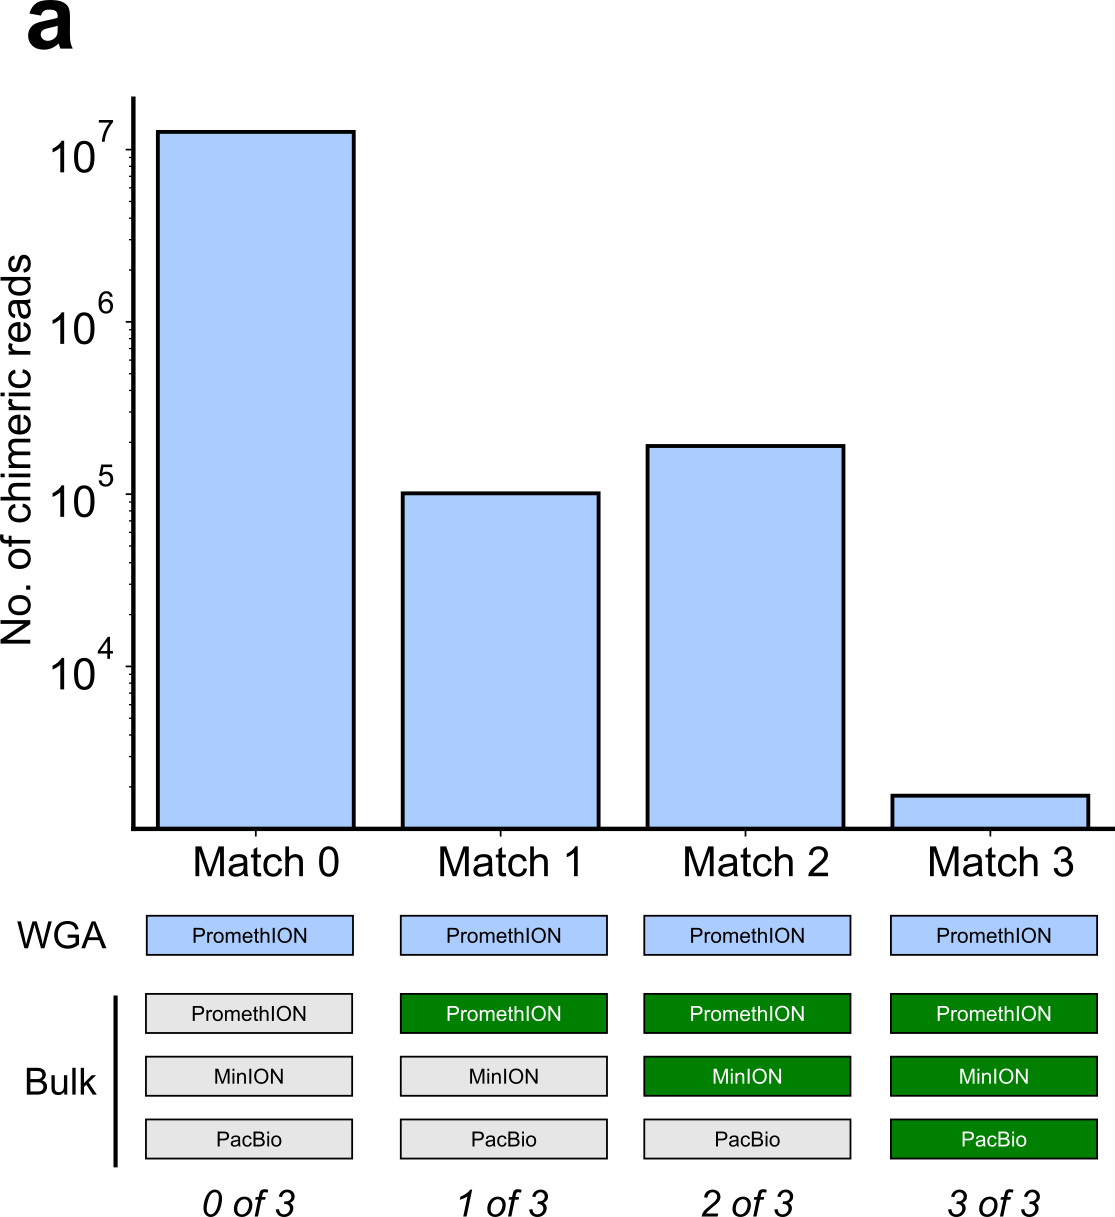
\includegraphics[width=0.8\textwidth]{final_figures/sf1}
	\end{center}
	\caption{{\bf Distribution of chimeric read matches between \gls{wga} and bulk sequencing datasets.}
		Bar chart showing the number of chimeric reads (y-axis, log scale) stratified by the number of matches found when comparing \gls{wga} chimeric reads against bulk sequencing data (x-axis). Match 0 indicates chimeric reads with no matches in bulk data (labeled as artificial chimeric artifacts, $\sim$10$^7$ reads). Match 1, 2, and 3 indicate chimeric reads with 1, 2, or 3 matches in bulk data respectively (labeled as biological reads, $\sim$10$^5$ reads each). This matching strategy forms the basis for ground truth labeling in supervised training.}\label{fig:sf1}
\end{figure}

\begin{figure}[!ht]
	\begin{center}
		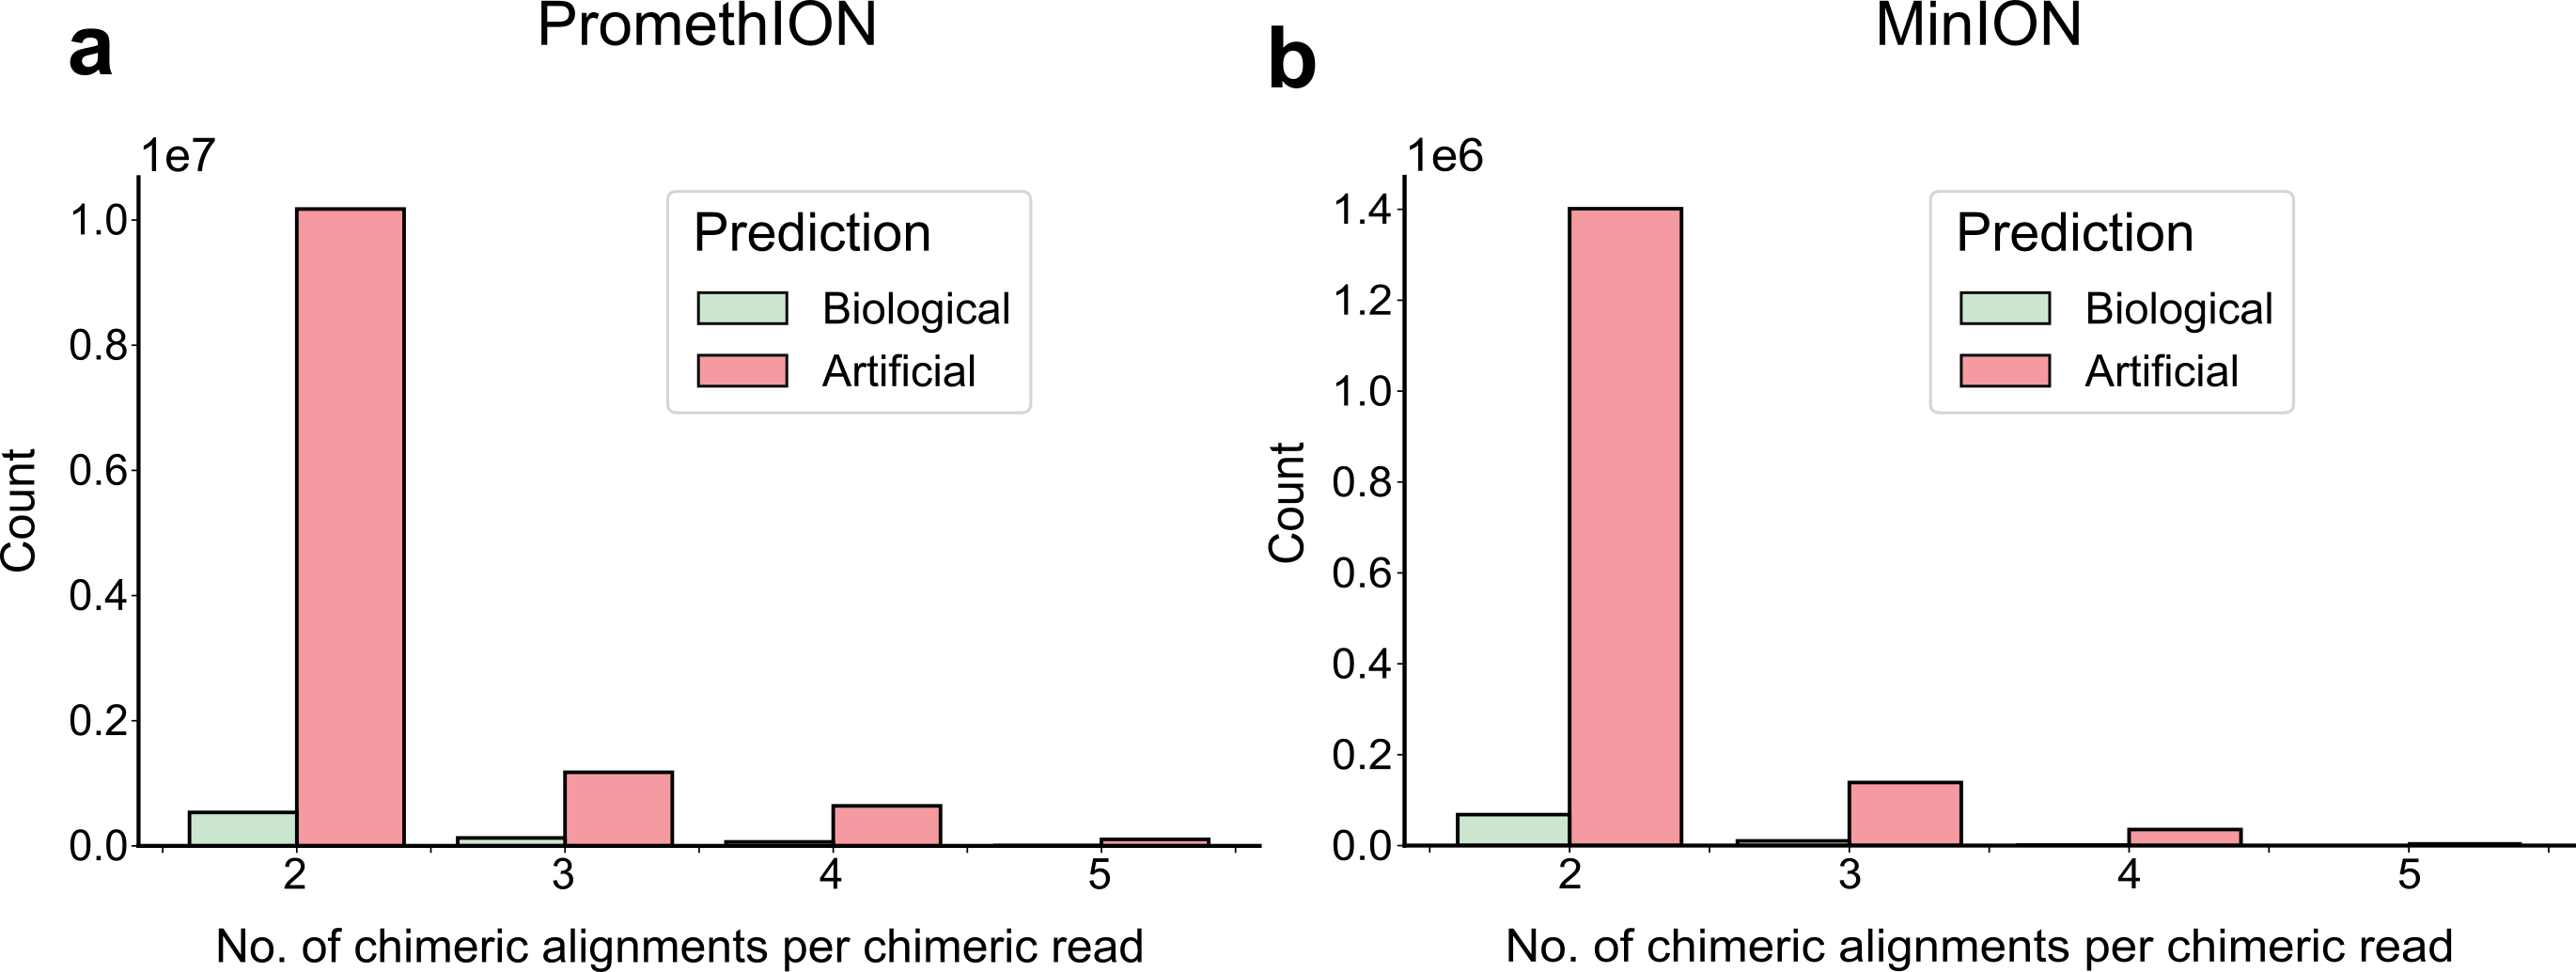
\includegraphics[width=\textwidth]{final_figures/sf2}
	\end{center}
	\caption{{\bf Distribution of chimeric alignments per chimeric read stratified by ChimeraLM prediction.}
		(a) PromethION P2 platform chimeric alignment analysis. Bar chart showing the distribution of chimeric reads based on the number of chimeric alignments per read (x-axis: 2, 3, 4+ alignments) and total read count (y-axis, log scale). Bars are colored by ChimeraLM's binary classification: biological (dark teal) and artificial (coral). Analysis includes only reads identified as chimeric (minimum 2 alignments per read).
		(b) MinION Mk1c platform chimeric alignment analysis. Bar chart showing the distribution of chimeric reads based on the number of chimeric alignments per read (x-axis: 2, 3, 4+ alignments) and total read count (y-axis, log scale). Bars are colored by ChimeraLM's binary classification: biological (dark teal) and artificial (coral). Analysis includes only reads identified as chimeric (minimum 2 alignments per read).}\label{fig:sf2}
\end{figure}

\begin{figure}[!ht]
	\begin{center}
		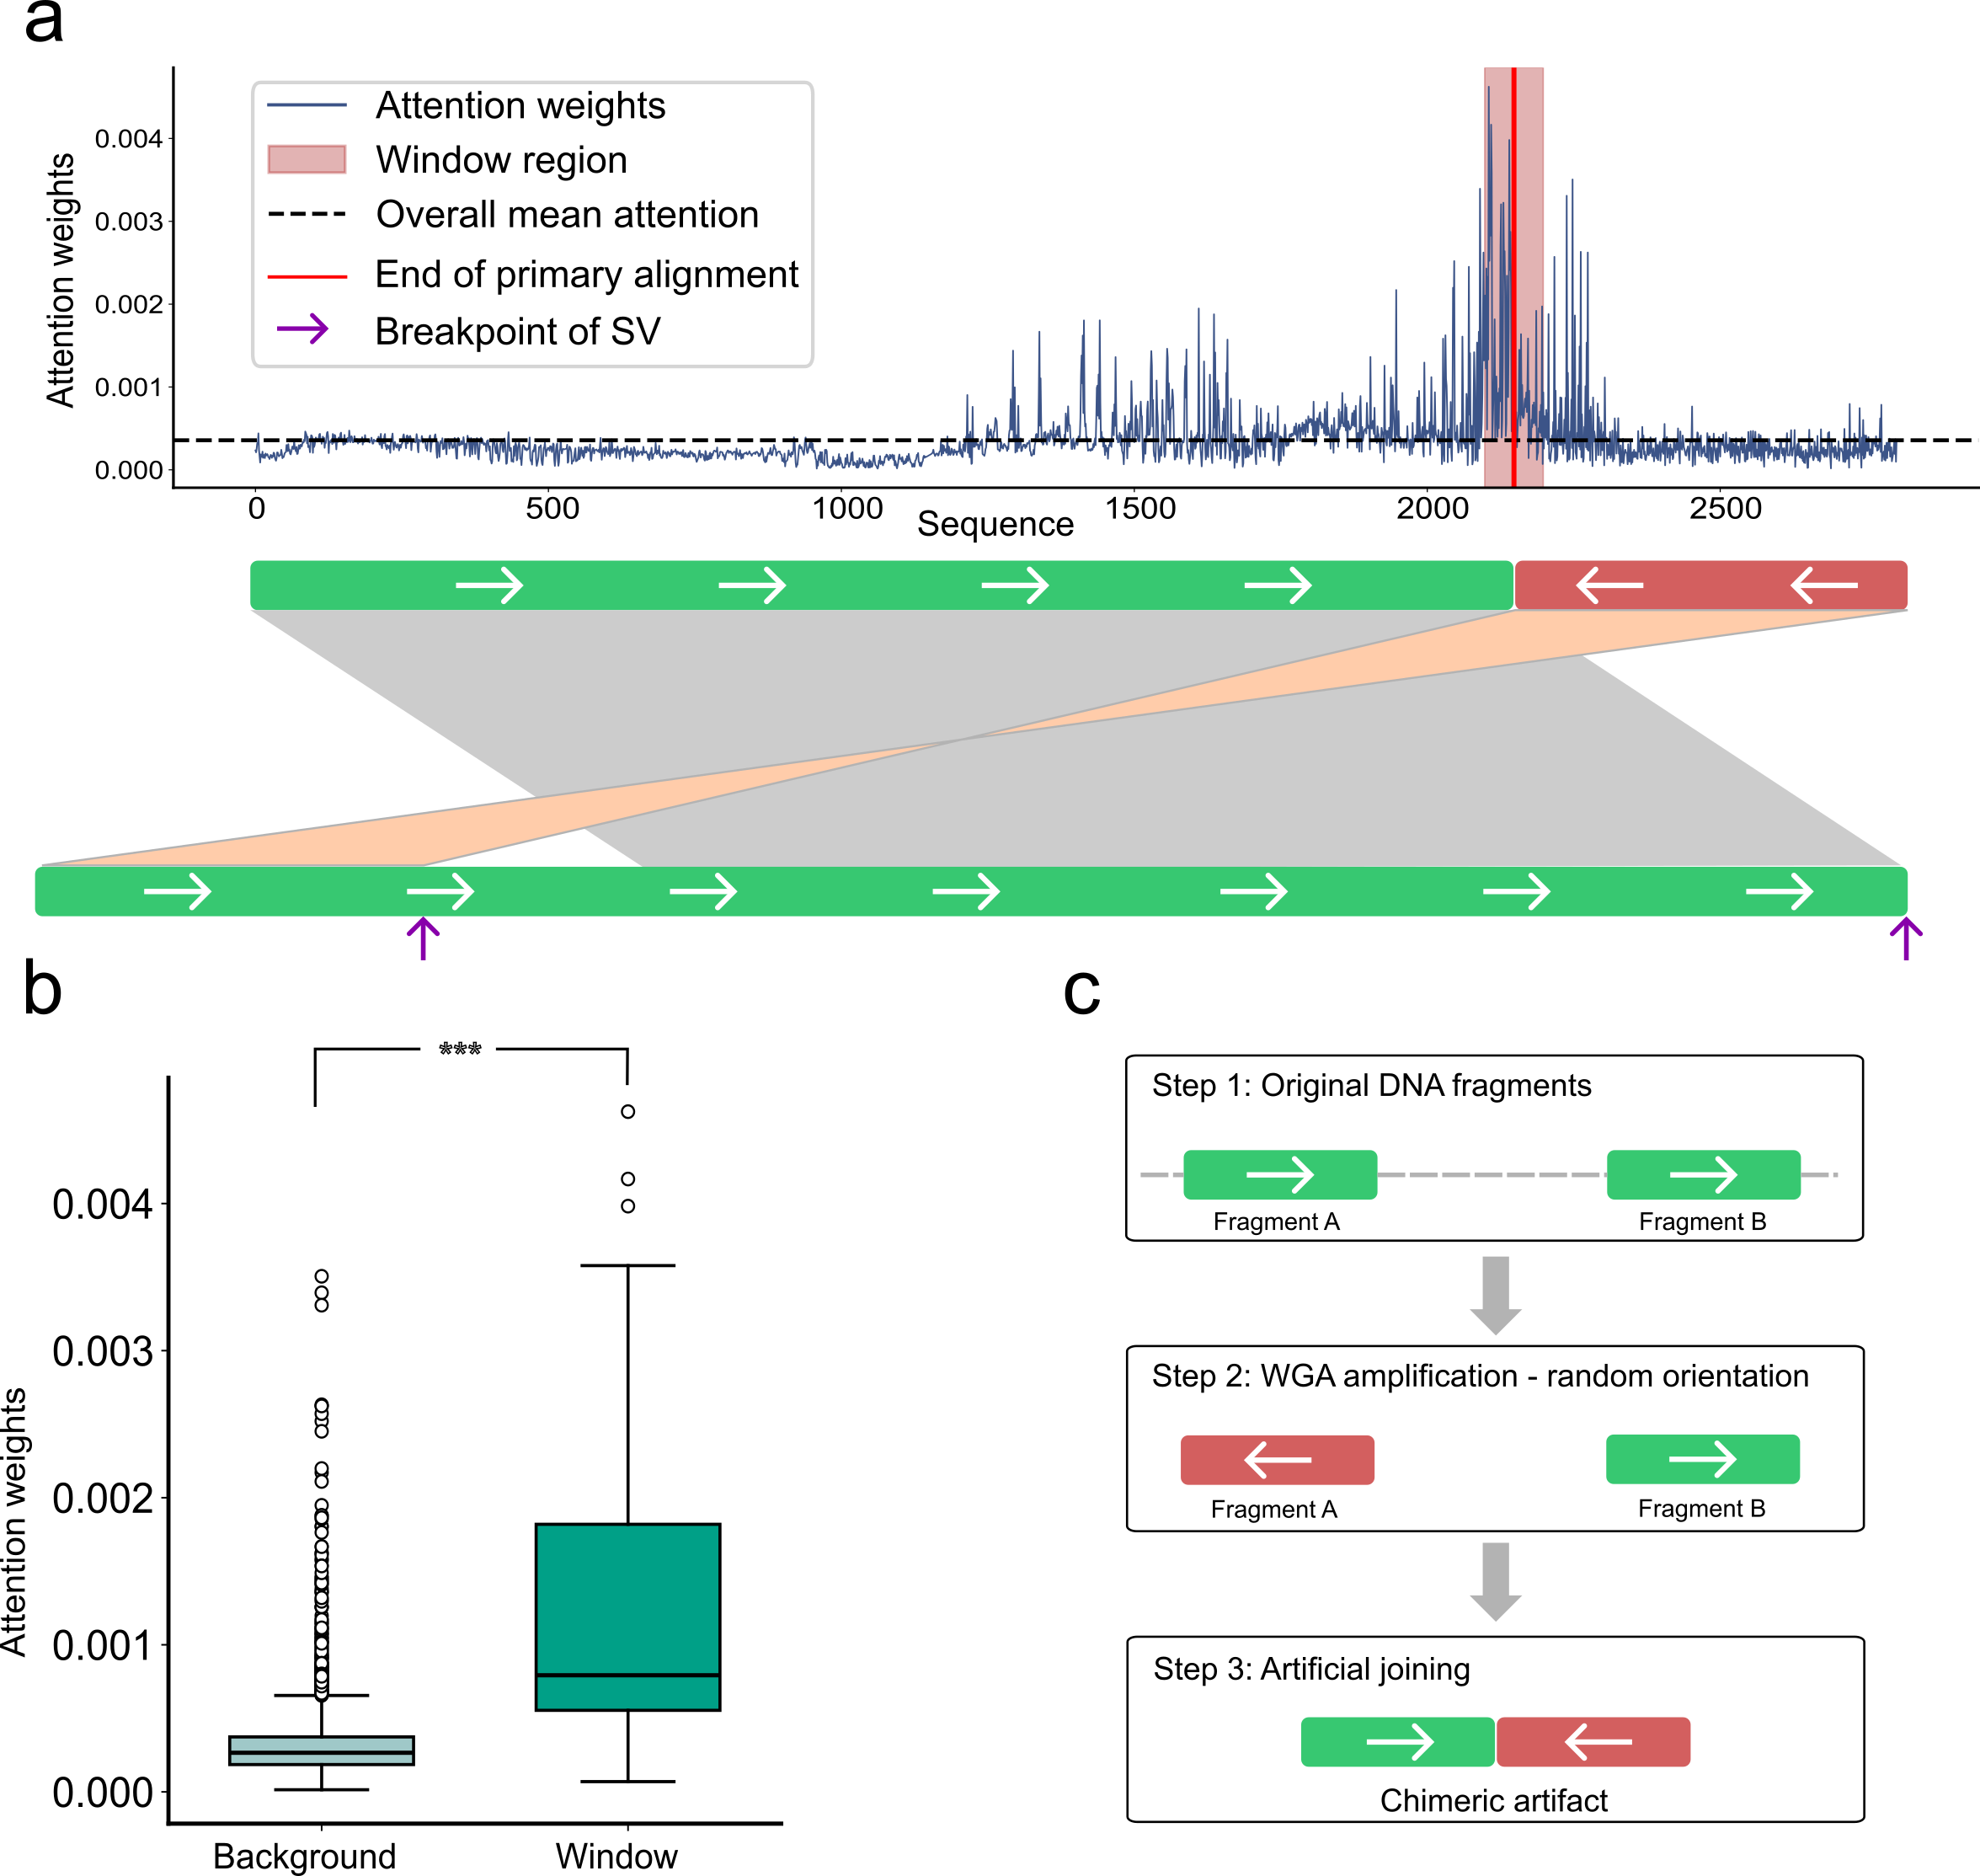
\includegraphics[width=\textwidth]{final_figures/sf3}
	\end{center}
	\caption{{\bf Additional example of attention-based interpretability showing ChimeraLM's focus on chimeric junction.}
		(a) Attention weight profile across another representative chimeric read. Upper panel shows attention weights per sequence position (blue line) with overall mean attention (dashed line). Red vertical line indicates the chimeric junction position in the read, with pink shading marking the junction window ($\pm$50 bp). Purple arrows indicate the corresponding \gls{sv} breakpoint positions in the reference genome. Lower panel illustrates read alignment: the read (top bar) shows forward sequence (green with rightward arrows) transitioning to reverse-complemented sequence (red with leftward arrows) at the junction. Reference genome (bottom bar) shows continuous forward orientation, with gray regions indicating alignment relationships.
		(b) Quantitative comparison of attention weights between junction window and background regions. Box plots show significantly elevated attention weights in the junction window compared to background regions, with statistical significance indicated (***, $p < 0.001$, Wilcoxon rank-sum test).
		(c) Chimera formation mechanism illustrated for this example. Step 1: Original DNA fragments from distant genomic loci (Fragment A and Fragment B) exist in forward orientation. Step 2: During \gls{wga}, Fragment A maintains forward orientation while Fragment B undergoes random reverse-complementation. Step 3: Template switching causes artificial joining of the two fragments with opposite orientations, creating a chimeric artifact.}\label{fig:sf3}
\end{figure}

\bmhead{Acknowledgements}

This project was supported in part by NIH grants R35GM142441 and R01CA259388 awarded to RY, and NIH grants R01CA256741, R01CA278832, and R01CA285684 awarded to QC.

\section*{Declarations}

\bmhead{Author Contributions}

YL, QG and RY designed the study.
YL and QG performed the analysis.
QG performed the experiments.
YL designed and implemented the model and computational tool.
YL, QG and RY wrote the manuscript.
RY supervised this work.

\bmhead{Data Availability}

\bmhead{Code Availability}

ChimeraLM, implemented in Python, is open source and available on GitHub (\url{https://github.com/ylab-hi/ChimeraLM}) under the Apache License, Version 2.0.
The package can be installed via PyPI (\url{https://pypi.org/project/chimeralm/}) using pip, with wheel distributions provided for Windows, Linux, and macOS to ensure easy cross-platform installation.
An interactive demo is available on Hugging Face (\url{https://huggingface.co/spaces/yangliz5/chimeralmr}), allowing users to test ChimeraLM\textquotesingle{s} functionality without local installation.
For large-scale analyses, we recommend using ChimeraLM on systems with \gls{gpu} acceleration. Detailed system requirements and optimization guidelines are available in the repository's documentation.

\bmhead{Conflict of interest}

RY has served as an advisor/consultant for Tempus AI, Inc. This relationship is unrelated to and did not influence the research presented in this study.

% Some journals require declarations to be submitted in a standardised format. Please check the Instructions for Authors of the journal to which you are submitting to see if you need to complete this section. If yes, your manuscript must contain the following sections under the heading `Declarations':

% \begin{itemize}
% 	\item Funding
% 	\item Conflict of interest/Competing interests (check journal-specific guidelines for which heading to use)
% 	\item Ethics approval and consent to participate
% 	\item Consent for publication
% 	\item Data availability
% 	\item Materials availability
% 	\item Code availability
% 	\item Author contribution
% \end{itemize}
%
% \noindent
% If any of the sections are not relevant to your manuscript, please include the heading and write `Not applicable' for that section.

\begin{appendices}

	\printglossaries

	% \section{Section title of first appendix}\label{secA1}
	%
	% An appendix contains supplementary information that is not an essential part of the text itself but which may be helpful in providing a more comprehensive understanding of the research problem or it is information that is too cumbersome to be included in the body of the paper.
	%
	%%=============================================%%
	%% For submissions to Nature Portfolio Journals %%
	%% please use the heading ``Extended Data''.   %%
	%%=============================================%%

	%%=============================================================%%
	%% Sample for another appendix section			       %%
	%%=============================================================%%

	%% \section{Example of another appendix section}\label{secA2}%
	%% Appendices may be used for helpful, supporting or essential material that would otherwise
	%% clutter, break up or be distracting to the text. Appendices can consist of sections, figures,
	%% tables and equations etc.
\end{appendices}

%%===========================================================================================%%
%% If you are submitting to one of the Nature Portfolio journals, using the eJP submission   %%
%% system, please include the references within the manuscript file itself. You may do this  %%
%% by copying the reference list from your .bbl file, paste it into the main manuscript .tex %%
%% file, and delete the associated \verb+\bibliography+ commands.                            %%
%%===========================================================================================%%

\bibliography{clean}% common bib file
%% if required, the content of .bbl file can be included here once bbl is generated
%%\input sn-article.bbl

\end{document}
